\documentclass[%
 reprint,
%superscriptaddress,
%groupedaddress,
%unsortedaddress,
%runinaddress,
%frontmatterverbose, 
%preprint,
%preprintnumbers,
nofootinbib,
%nobibnotes,
%bibnotes,
 amsmath,amssymb,
 aps,
%pra,
%prb,
%rmp,
%prstab,
%prstper,
floatfix,
]{revtex4-2}

\usepackage{graphicx}% Include figure files
\usepackage{dcolumn}% Align table columns on decimal point
\usepackage{bm}% bold math
\usepackage[colorlinks=false,pdfstartview=FitV,linkcolor=black,citecolor=black,urlcolor=black]{hyperref}% add hypertext capabilities
\usepackage[mathlines]{lineno}% Enable numbering of text and display math
\usepackage{placeins}% control float placement with \FloatBarrier
%\linenumbers\relax % Commence numbering lines
\extrafloats{75}

\iffalse
\setcounter{topnumber}{8}
\setcounter{bottomnumber}{8}
\setcounter{totalnumber}{16}
\setcounter{dbltopnumber}{8}
\renewcommand{\topfraction}{0.95}
\renewcommand{\bottomfraction}{0.95}
\renewcommand{\textfraction}{0.02}
\renewcommand{\floatpagefraction}{0.75}
\renewcommand{\dbltopfraction}{0.95}
\renewcommand{\dblfloatpagefraction}{0.75}
\setlength{\floatsep}{6pt plus 2pt minus 2pt}
\setlength{\textfloatsep}{8pt plus 2pt minus 2pt}
\setlength{\intextsep}{6pt plus 2pt minus 2pt}
\fi

\begin{document}

\preprint{APS/123-QED}

\title{A Computational Model of Bound and Pseudo-Bound States in the Yukawa Potential}
%\thanks{A footnote to the article title} %

\author{Charles~J.~Mikolajczak}
  \email{cmikolajczak@umassd.edu}

\author{Jianyi~J.~Wang}%
  \email{jwang@umassd.edu}

  \affiliation{
  Physics Department, University of Massachusetts, N. Dartmouth, MA 02747
}

\iffalse
\author{Charlie Author}
  \homepage{http://www.Second.institution.edu/~Charlie.Author}
\affiliation{
  Second institution and/or address\\
  This line break forced% with \\
}%
\affiliation{
  Third institution, the second for Charlie Author
}%
\author{Delta Author}
\affiliation{%
 Authors' institution and/or address\\
 This line break forced with \textbackslash\textbackslash
}%
\fi

%\collaboration{CLEO Collaboration}%\noaffiliation

\date{\today}

% =========
% Abstract
% =========
\begin{abstract}
{
  The Yukawa potential is a short-range interaction proposed by Hideki Yukawa in 1935 to describe the strong nuclear force through the proposal of a massive particle, later identified as the meson. 
  His proposal explains how the meson mediates the attractive force between nucleons and overcomes the repulsive electromagnetic force at short distances, contributing to the stability of atomic nuclei. 
  This model acts as a screened Coulomb potential with a similar $1/r$ dependence, acting over distances on the order of $10^{-15}$ m (1 fm), but with an exponential screening factor of $e^{-\lambda r}$. 
  We aim to build a computational solver exploring bound and pseudo-bound states by solving the non-relativistic radial Schr\"odinger equation. 
  The main focus is to solve for low-energy bound and pseudo-bound state eigenenergies and eigenfunctions using numerical methods and to plot the corresponding wavefunctions as functions of radial distance $r$. 
  These bound and pseudo-bound states form and are dependent on varying system parameters, such as potential well depth and width, as well as screening strength. 
  For example, as the potential well depth increases, more bound states appear. 
  We aim to examine how these states depend on the strength and range of the parameters, and identify the conditions under which bound and pseudo-bound states emerge and disappear.
}
\end{abstract}


%\keywords{Suggested keywords}%Use showkeys class option if keyword
                              %display desired
\maketitle

%\tableofcontents


%\iffalse
% ==============
% Intro Section
% ==============
\section{\label{sec:intro}Introduction}

%\iffalse
% -----------
% Background
% -----------
%\subsection{\label{subsec:background}Background}
{
  A bound state is one where the total energy of the state is negative. 
  This is predominantly seen in the Hydrogen system, where all states are bound (Fig. \ref{fig:5}). 
  Pseudo-bound states are states that have positive energies and behave like bound states, however because of that positive energy, there is a probability a particle in that state can tunnel through the potential barrier. 
  By exploring where these bound and pseudo-bound states live, we can then determine the behavior of systems that allow scattering to occur. 
  The model used for this exploration is the Yukawa potential.

  The system being modeled is one of the early theoretical models of the strong nuclear force. 
  Taking the form 
  \begin{equation}
    V(r) = \pm g^2 \frac{e^{-\lambda r}}{r}, \label{eq:1}
  \end{equation}
  in the initial submission of the paper \cite{yuk1935}, where $\lambda$ is the screening parameter and $g$ is the coupling constant, this assumes the potential to be of a similar shape to the electromagnetic Coulomb force, described similarly by a factor $1/r$, as well as being a central field. 
  The key difference between these two potentials is the exponential factor $e^{-\lambda r}$, acting as a screened Coulomb variant, describes an exponentially decaying potential (i.e., the Yukawa tail) approaching zero much quicker than the standard Coulomb model. 
  However, if we take this to be the description of the strong nuclear force, a fundamental concept must be considered. 
  
  The electromagnetic force is seen to be attractive\footnote{The indicator regarding whether or not a system is attractive or repulsive lies in the sign of the potential. A positive potential energy signals a repulsive force, whereas a negative potential energy describes an attractive force.} between particles of opposite charges and repulsive for those of similar charges. 
  We now consider two nucleons of the same charge, the proton. 
  Interacting attractively inside the range of nuclear radius ($r \leq 1 \text{ fm}$) and repulsively outside ($r > 1 \text{ fm}$), we are able to create a simple model that behaves as such while keeping the form of the initial Yukawa potential.
  We use the modified Yukawa potential, described by 
  \begin{equation}
    V(r) = \Bigg\{
      \begin{matrix}
        -V_0, \hspace{0.25cm} r \leq R \\
        \frac{e^{-\lambda r}}{r}, \hspace{0.25cm} r > R
      \end{matrix}, \label{eq:2}
  \end{equation}
  with $V_0$ being the depth of a spherical potential well and $R$ is the radial position associated with the boundary where the potential swaps from the attractive nuclear force to a repulsive Coulomb-like force. 
  This modified potential allows us to approximate the behavior of the system as a piecewise function, a combination of a spherical potential well from $0 < r \leq R$ and the Yukawa tail for $r > R$. 
  This form eases conceptualization while also giving an approximate physical interpretation of the system, creating a model to center around while calculating the eigenenergies and eigenfunctions for the system. 
  While finding the energies and wave functions, we vary the parameters $\lambda$, $V_0$, and $R$ to explore how bound and pseudo-bound states depend on these parameters.
}
%\fi


%\iffalse
% ================
% Methods Section
% ================
\section{\label{sec:methods}Methods}

%\iffalse
% -----
% Math
% -----
\subsection{\label{subsec:math}Mathematics}
{
  We begin by using the reduced radial Schr\"odinger equation \cite{griffithsqm2} for a central potential, given by
  \begin{equation}
    -\frac{\hbar^2}{2m} \frac{d^2}{dr^2} u_{n\ell}(r) + \bigg[V(r) + \frac{\hbar^2 \ell(\ell + 1)}{2 m r^2} \bigg] u_{n\ell}(r) = E u_{n\ell}(r), \label{eq:3}
  \end{equation}
  where $u_{n\ell}(r) = r R_{n\ell}(r)$ is the reduced radial wave function, $m$ is the mass of the system, $n$ is the principal quantum number, $\ell$ is the orbital angular momentum quantum number, and $E$ is the total energy of the system. 
  We will use $u_{n\ell}(r) = u_{n\ell}$ to simplify notation. 
  We will also define the effective potential to be
  \begin{equation}
    V_{\text{eff}}(r) = V(r) + \frac{\hbar^2 \ell(\ell + 1)}{2 m r^2}. \label{eq:4}
  \end{equation}
  For the same purpose as $u_{n\ell}$, we'll use $V_{\text{eff}} (r) = V_{\text{eff}}$. 
  The potential $V(r)$ is as defined in Eq. (\ref{eq:2}), and the latter half of $V_{\text{eff}}$ is the centrifugal term of the potential energy, which arises from the angular momentum of the system. 
  Eq. (\ref{eq:4}) now becomes 
  \begin{equation}
    -\frac{\hbar^2}{2m} \frac{d^2}{dr^2} u_{n\ell} + (V_{\text{eff}}) u_{n\ell} = E u_{n\ell}, \label{eq:5}
  \end{equation}
  and we can simplify the equation further by using atomic units (a.u.), where $\hbar = m = 1$, giving us
  \begin{equation}
    -\frac{1}{2} \frac{d^2}{dr^2} u_{n\ell} + (V_{\text{eff}}) u_{n\ell} = E u_{n\ell}. \label{eq:6}
  \end{equation}
  If we take $V_{\text{eff}}(r)$ to be a known function, we can use the Numerov method to solve the Schr\"odinger equation numerically.

  The Numerov method is of the form 
  \begin{equation}
    u'' + f(x) u = 0, \label{eq:7}
  \end{equation}
  where $f(x)$ is a known function.
  By rearranging Eq. (\ref{eq:6}), we obtain the Numerov form of the Schr\"odinger equation
  \begin{equation}
    \frac{d^2}{dr^2} u_{n\ell} + 2(E - V_{\text{eff}}) u_{n\ell} = 0. \label{eq:8}
  \end{equation}
  This form of the reduced radial Schr\"odinger equation is implemented in the computational solver, allowing for the use of the three-term recursive formula for updating $u$ in Eq.(\ref{eq:9})
  \begin{widetext}
  \begin{equation}
    u_{i+1} = \Big(1 + \frac{h^2}{12}f_{i+1} \Big)^{-1} \Big[2 \Big(1 - \frac{5 h^2}{12}f_i \Big)u_i - \Big(1 + \frac{h^2}{6}f_{i-1} \Big)u_{i-1}\Big] + \mathcal{O}(h^6), \label{eq:9}
  \end{equation}
  \end{widetext}
  where $h$ is the step size of the discretized radial grid, $i$ indicating the iteration, and $\mathcal{O}(h^6)$ representing the error on the order of $h^6$. 
  We can see indices of $i-1$, $i$, and $i+1$, each indicating the value from the previous iteration, current iteration, and updated value, respectively. 
  The Numerov method is particularly helpful because it is a method for solving 2nd Order Linear ODEs with only the 2nd derivative. 
  As we can see in Eq. (\ref{eq:8}), the rearranged Schr\"odinger equation satisfies this condition, as $E$ and $V_{\text{eff}}$ are considered here to be scalar values instead of operators. 
}
%\fi

%\iffalse
% ------------
% Computation
% ------------
\subsection{\label{subsec:computation}Computational Setup}
{
  We use \texttt{hydrogen.py}\footnote{Taken from \cite{WangCP}~Ch.~9, App.~C as Program Listing 9.5. Source code for this program can be found \href{https://github.com/com-py/compy/blob/master/ch09/Program_9.5_hydrogen.py}{here}.} as a foundation for the project, already implementing the Numerov form from Eq. (\ref{eq:8}). 
  This code models the Hydrogen system, this model is based in a.u., using $E_0$ as the unit of energy and $a_0$\footnote{$a_0 \equiv$ Bohr Radius. The value in SI units is $a_0 = 0.5 \times 10^{-10}$ m.} being the unit of length. 
  Because of such a large difference between atomic to nuclear radial scales, the energy values must be scaled, as well. 

  \begin{equation}
      E_0 = \frac{e^2}{4\pi \varepsilon_0 a_0} \propto \frac{1}{a_0} = \frac{1}{0.5 \times 10^{5}}
      \label{eq:10}
    \end{equation}

  \begin{equation}
      E^* = a_0 E_0 = (0.5 \times 10^{5})E_0
      \label{eq:11}
  \end{equation}

  We introduce $E^*$ in Eq. (\ref{eq:11}) to account for the scale change in length. 
  
  As stated before, we use the Numerov method as our ODE solver. 
  We also make use of the shooting method, as seen in Eq. (\ref{eq:12}). 
  
  \begin{equation}
    f(E) = u_m^\downarrow w_m^\uparrow - u_m^\uparrow w_m^\downarrow, \hspace{0.25cm} w = u'
    \label{eq:12}
  \end{equation}

  By using the shooting method, we are able to approximate the wave function by matching them at the piecewise break $R$. 
  We denote outward integration (integrating\footnote{Because of the nature of the potential, we cannot evaluate at $r = 0$, therefore using an approximate value of $10^{-6}$.} from $10^{-6}$ to $R$) with $\uparrow$ and inward integration (integrating from $r_{\text{max}}$ to $R$) with $\downarrow$. 
  Using both $u$ and $w$ makes sure the wave functions are smooth and continuous. 
  We combine the use of the shooting method with a rootfinder, the bisection method. 
  The bisection method uses roots of the shooting function to approximate our energies. 

  The programming language used in the script is Python, using Python 3.12. 
  Our initial parameter values are $V_0 = 20E^*$, $R = 2$ fm, and $\lambda = 0.2$. 
  These are the parameters for the plots in Section \ref{sec:results}. 
  We set up the main calculation of energies and wave functions as a \texttt{while} loop (from $V_0$ to $e^{-\lambda r}/r$) nested inside a \texttt{for} loop over $\ell$. 
  The wave functions get stored in two lists, one for upward integration and one for downward integration, then get concatenated. 
  Energy values also get stored in a list, getting appended once found. 
  Plotting is done using the \texttt{matplotlib} package, using the \texttt{colormaps} module for color-coding. 
}
%\fi

%\fi % section


%\iffalse
% ================
% Results Section
% ================
\section{\label{sec:results}Results}

%\iffalse
% -----------------
% Potential Energy
% -----------------
\subsection{\label{subsec:potential}Potential Energy}
{
  The first result to consider is the potential energy. 
  As seen in Eq. (\ref{eq:4}), $V_{\text{eff}}$ is dependent on both $r$ and $\ell$.
  In the Hydrogen system, the potential for $\ell = 0$ describes an attractive force, with $V_{\text{eff}} = V(r) = -1/r$. 
  However, for $\ell \neq 0$, the behavior for $r \rightarrow 0$ becomes dominated by the centrifugal term. 
  The comparison between the two contributions can be seen in Fig. (\ref{fig:1}). 
  
  \begin{figure}[!htbp]
    \centering
    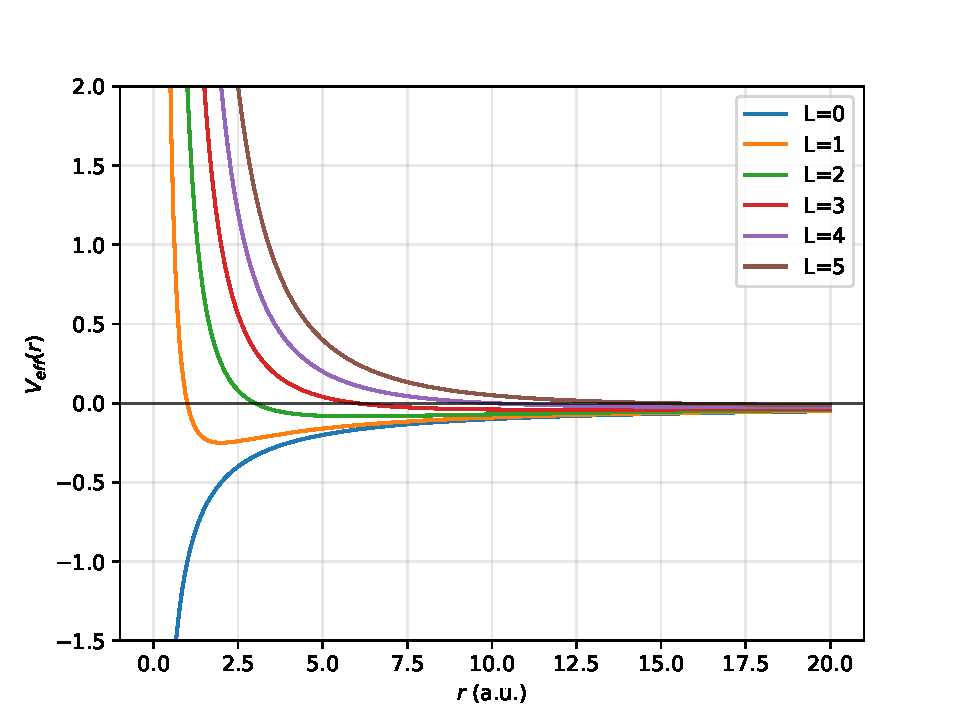
\includegraphics[width=1.0\linewidth]{plots/potential/h_eff_pot.pdf}
    \caption{Effective Coulomb potential $V_{\text{eff}}$ for $\ell = 0,1,2,3,4,5$.}
    \label{fig:1}
  \end{figure}

  This is similar to $V_{\text{eff}}$ for the Yukawa potential. 
  For $\ell = 0$, $V_{\text{eff}} = V(r)$, creating the plot associated with Eq. (\ref{eq:2}).

  \begin{figure}[!htbp]
    \centering
    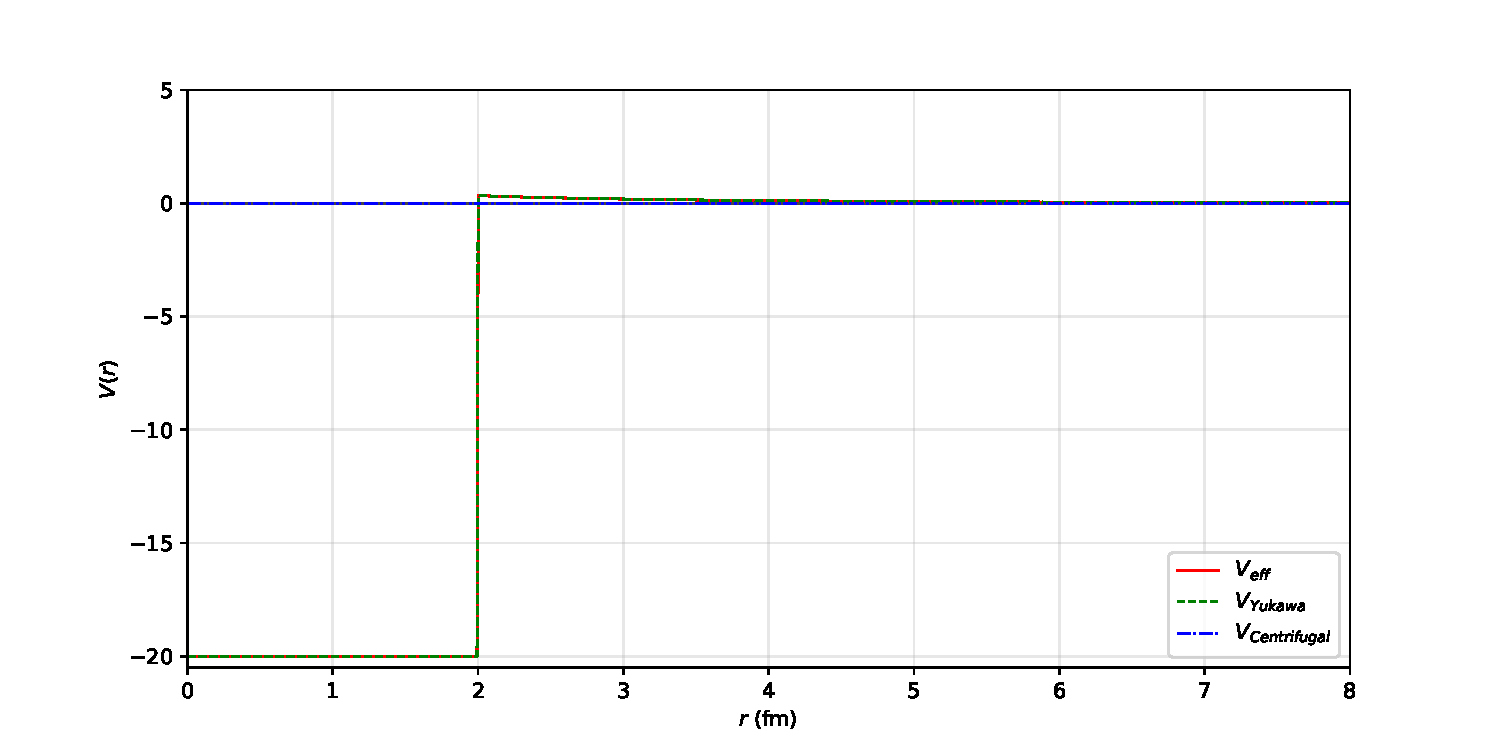
\includegraphics[width=1.0\linewidth]{plots/potential/3/pb_Vr_L0.pdf}
    \caption{Effective Yukawa potential $V_{\text{eff}}$ for $\ell = 0$.}
    \label{fig:2}
  \end{figure}

  For $\ell = 0$, the pieces of $V(r)$ each have the centrifugal term added to them in their respective regions, the term's increasing influence as $\ell$ increases. 
  Figs. (\ref{fig:3}) and (\ref{fig:4}) show this influence as $\ell$ increases, particularly in the finite well. 

  \begin{figure}[!htbp]
    \centering
    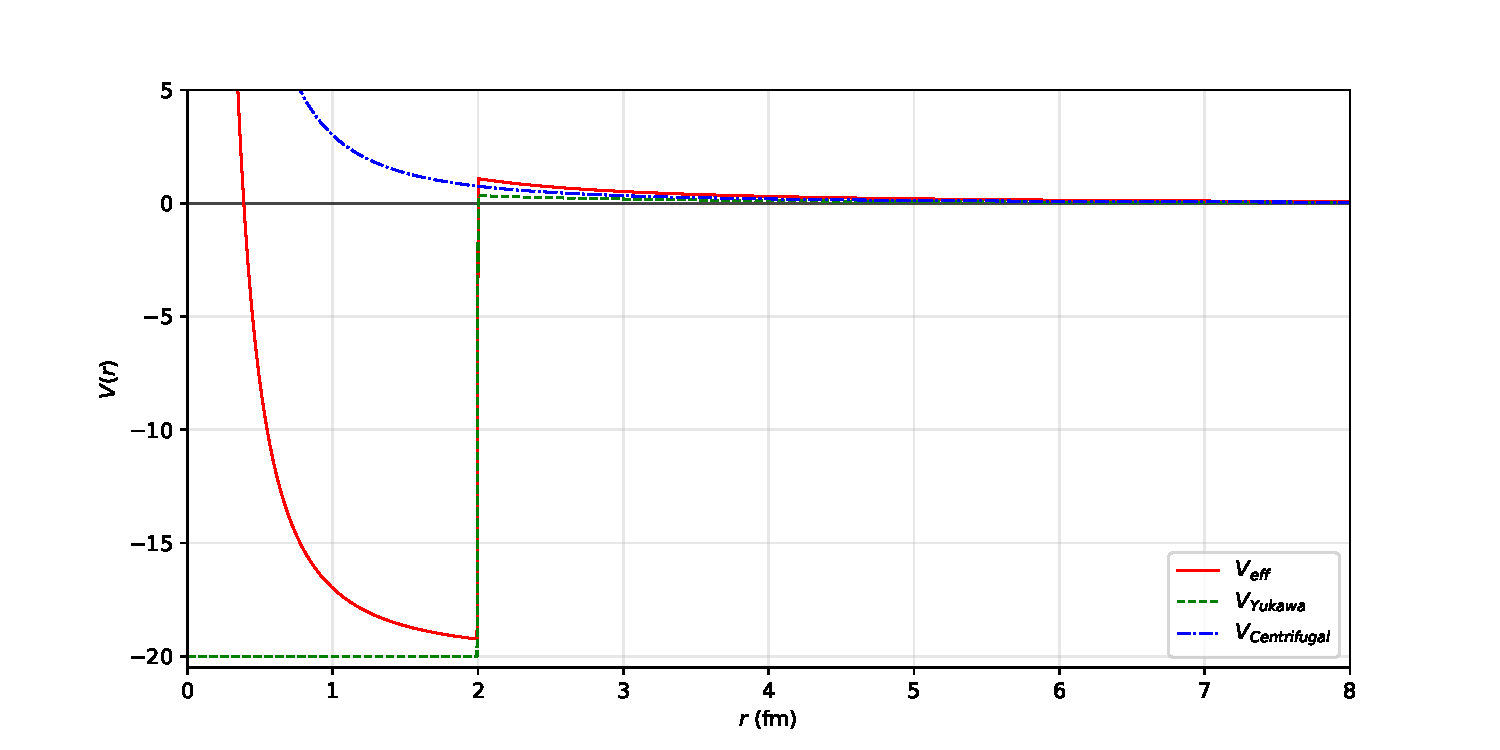
\includegraphics[width=1.0\linewidth]{plots/potential/3/pb_Vr_L2.pdf}
    \caption{Effective Yukawa potential $V_{\text{eff}}$ for $\ell = 2$.}
    \label{fig:3}
  \end{figure}

  \begin{figure}[!htbp]
    \centering
    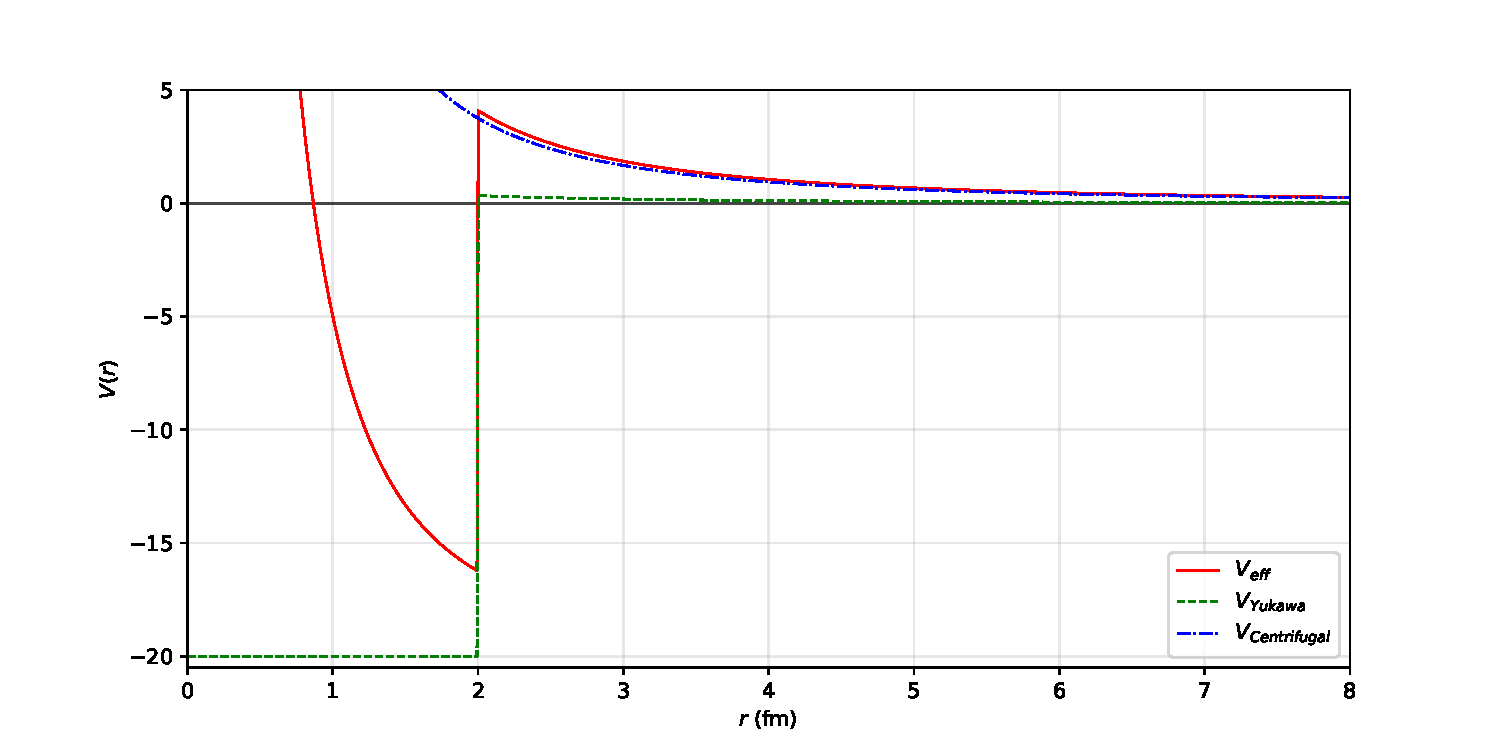
\includegraphics[width=1.0\linewidth]{plots/potential/3/pb_Vr_L5.pdf}
    \caption{Effective Yukawa potential $V(r)$ for $\ell = 5$.}
    \label{fig:4}
  \end{figure}
    
  Because the finite well region of the pure Yukawa potential is of constant value, the centrifugal term dominates more heavily in that region. 
  This causes $V_{\text{eff}}$ to have a similar shape to the centrifugal potential in the region of the well, just shifted down by 20 units. 
}
%\fi

%\iffalse
% -------------
% Total Energy
% -------------
\subsection{\label{subsec:energy}Total Energy}
{
  By plotting the energy levels, we can see exactly which states are purely bound and which are pseudo-bound. 
  Fig. (\ref{fig:5}) illustrates the eigenenergies for the Hydrogen atom, with the $n$--values separated by color. 
  We can see these states are degenerate, meaning the energies for the same $n$--value but differing $\ell$--values are the same. 

  \begin{figure}[!htbp]
    \centering
    
\includegraphics[width=\linewidth]{plots/energy/H_energy.pdf}
    \caption{Hydrogen Energy from $\ell = 0$ to $\ell = 5$.}
    \label{fig:5}
  \end{figure}

  Fig. (\ref{fig:6}) shows the eigenenergies for particles in the Yukawa potential, with the same color-coding as Fig. (\ref{fig:5}). 
  There's an immediate difference, showing a downward slant in $n$--valued bound state energies. 
  This slant represents the lifting of degeneracy, making the energy $E$ dependent on both $n$ and $\ell$. 
  There is another major difference: positive energies. 
  These positive energies are representative of pseudo-bound and scattering states. 
  We will look at these more closely in Section \ref{subsec:wfs-and-pds}.

  \begin{figure}[!htbp]
    \centering
    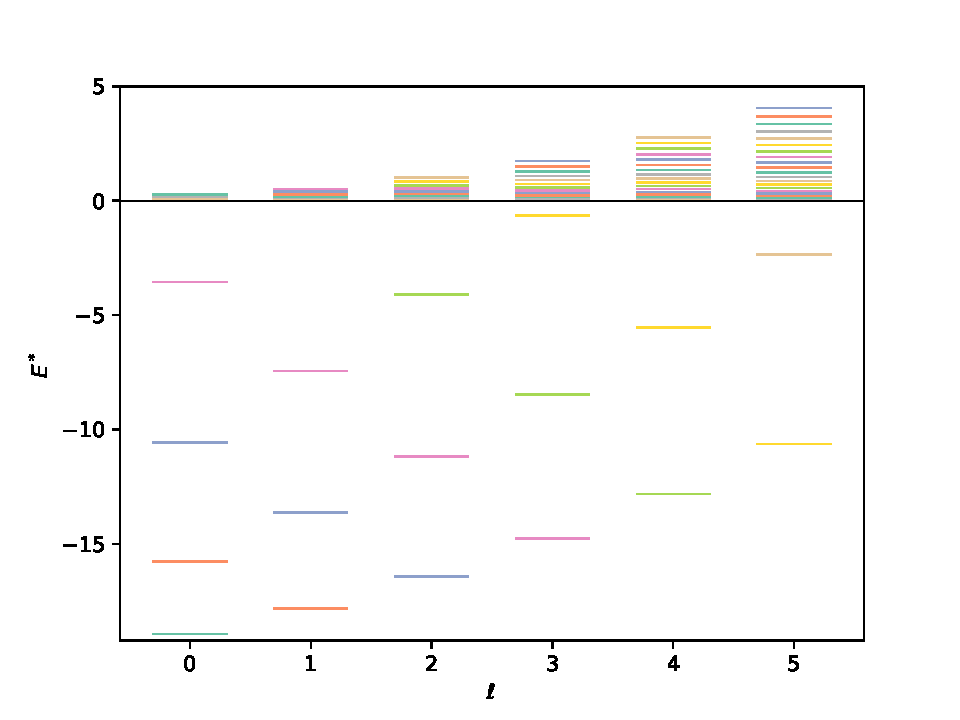
\includegraphics[width=\linewidth]{plots/energy/3/pb_energy.pdf}
    \caption{Yukawa Energy from $\ell = 0$ to $\ell = 5$.}
    \label{fig:6}
  \end{figure}
}
%\fi

%\iffalse
% ------------
% WFs and PDs
% ------------
\subsection{\label{subsec:wfs-and-pds}Wave Functions and Probability Densities}
{
  Fig. (\ref{fig:7}) shows the reduced radial wave function for the ground state, and Fig. (\ref{fig:8}) the associated probability density. 
  We can see there are no nodes, and the probability of this state being bound is very high. 
  This is exactly what is expected conceptually. 

  \begin{figure}[!htbp]
    \centering
    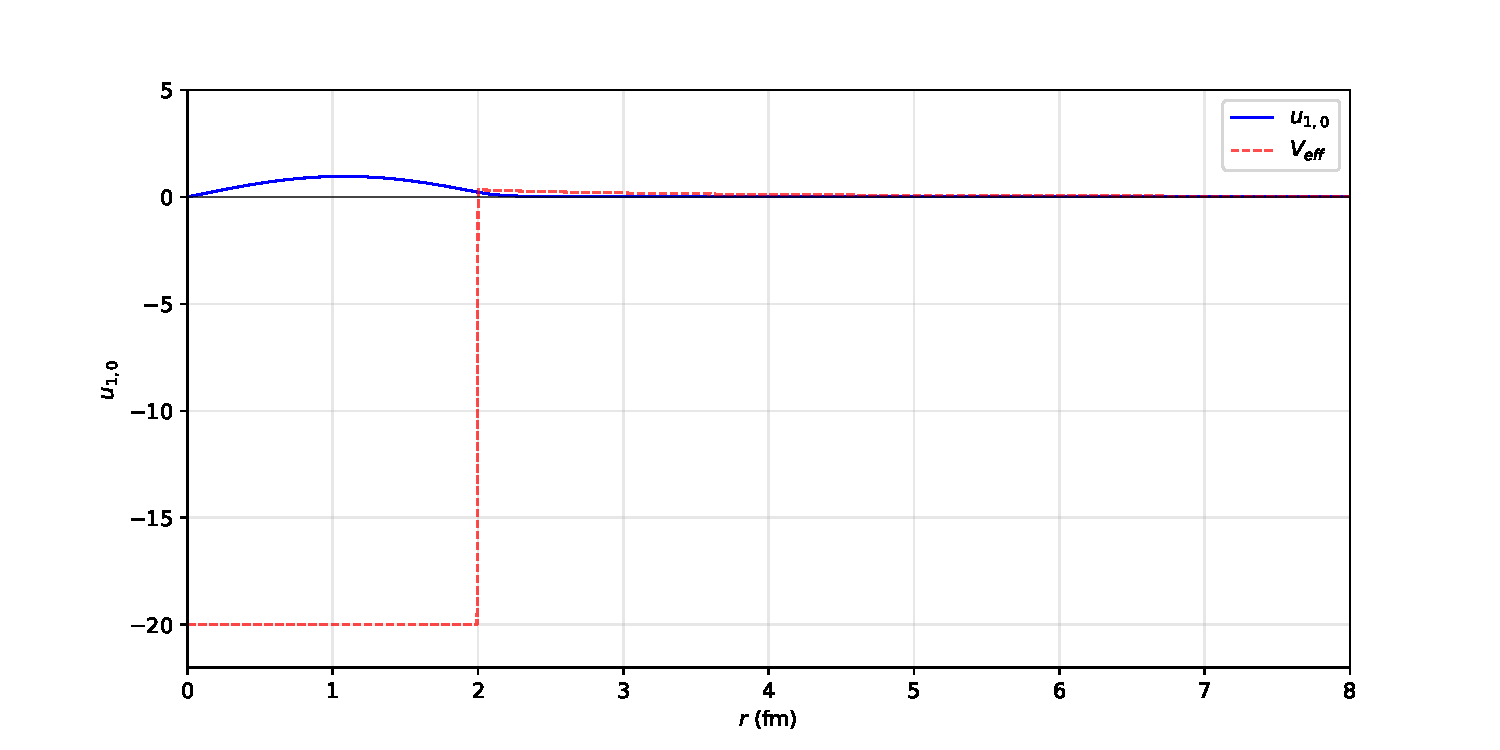
\includegraphics[width=\linewidth]{plots/wfs-and-pds/3/pb_wf_u10.pdf}
    \caption{Reduced radial wave function for $n = 1$, $\ell = 0$, the ground state.}
    \label{fig:7}
  \end{figure}

  \begin{figure}[!htbp]
    \centering
    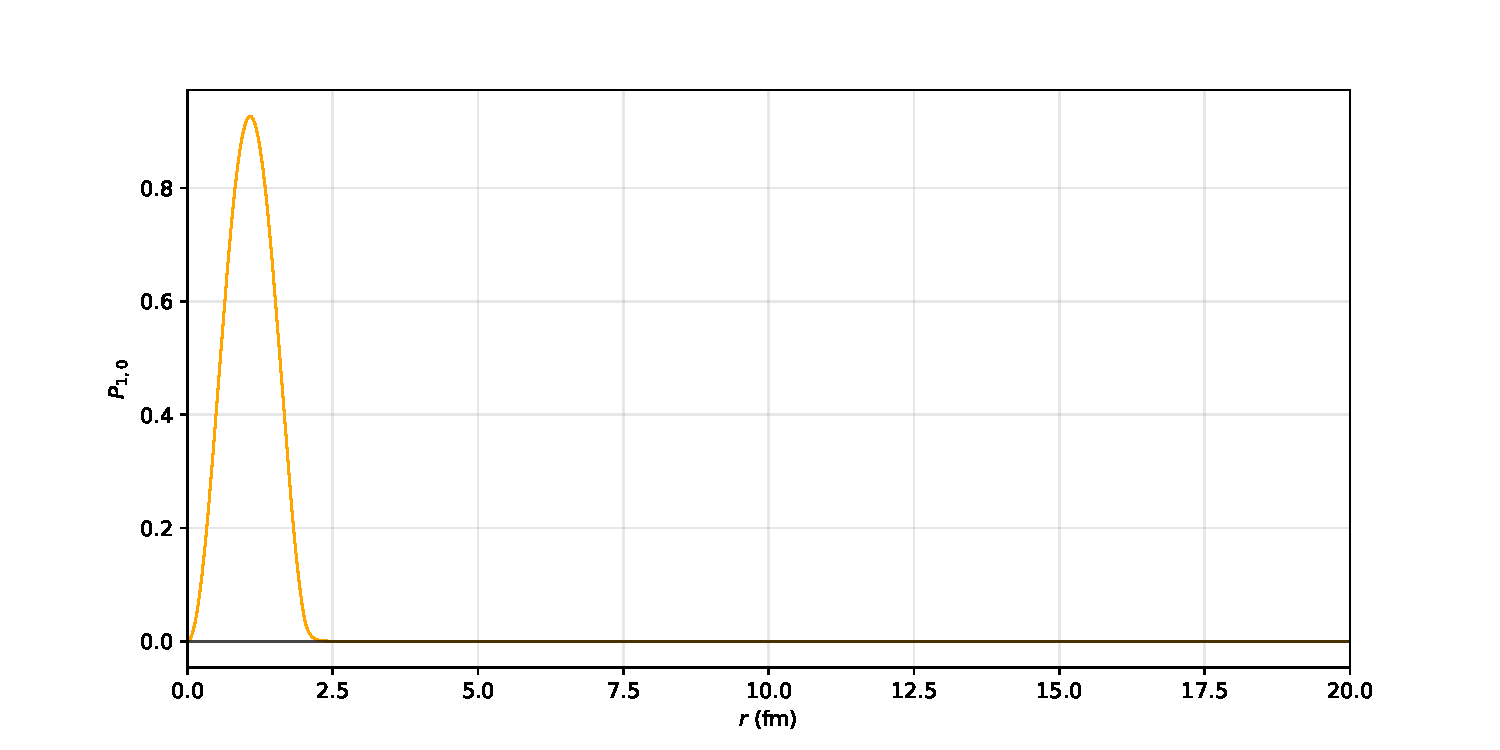
\includegraphics[width=\linewidth]{plots/wfs-and-pds/3/pb_pd_u10.pdf}
    \caption{Probability density $\mathcal{P}_{1,0}$ for $n = 1$, $\ell = 0$, the ground state.}
    \label{fig:8}
  \end{figure}

  For more interesting results, we focus on the $u_{6,3}$, $u_{7,5}$, and $u_{25,5}$ states. 
  Comparing Figs. (\ref{fig:9}) and (\ref{fig:12}), we can see the wave function for $u_{6,3}$ has one more node than for $u_{7,5}$. 
  We can see a pattern between the relationships of $n$, $\ell$, and the number of nodes. 
  Explicitly laying out this relationship gives

  \begin{equation}
    \text{\# of nodes} = n - \ell - 1\footnote{This relationship is only for the reduced radial wave functions.}.
  \end{equation}

  So, even though the state $u_{7,5}$ has a higher energy, the number of nodes is only dependent on the quantum numbers. 
  We can see the probability of these two states being bound is once again high, as it was with the ground state. 

  \begin{figure}[!htbp]
    \centering
    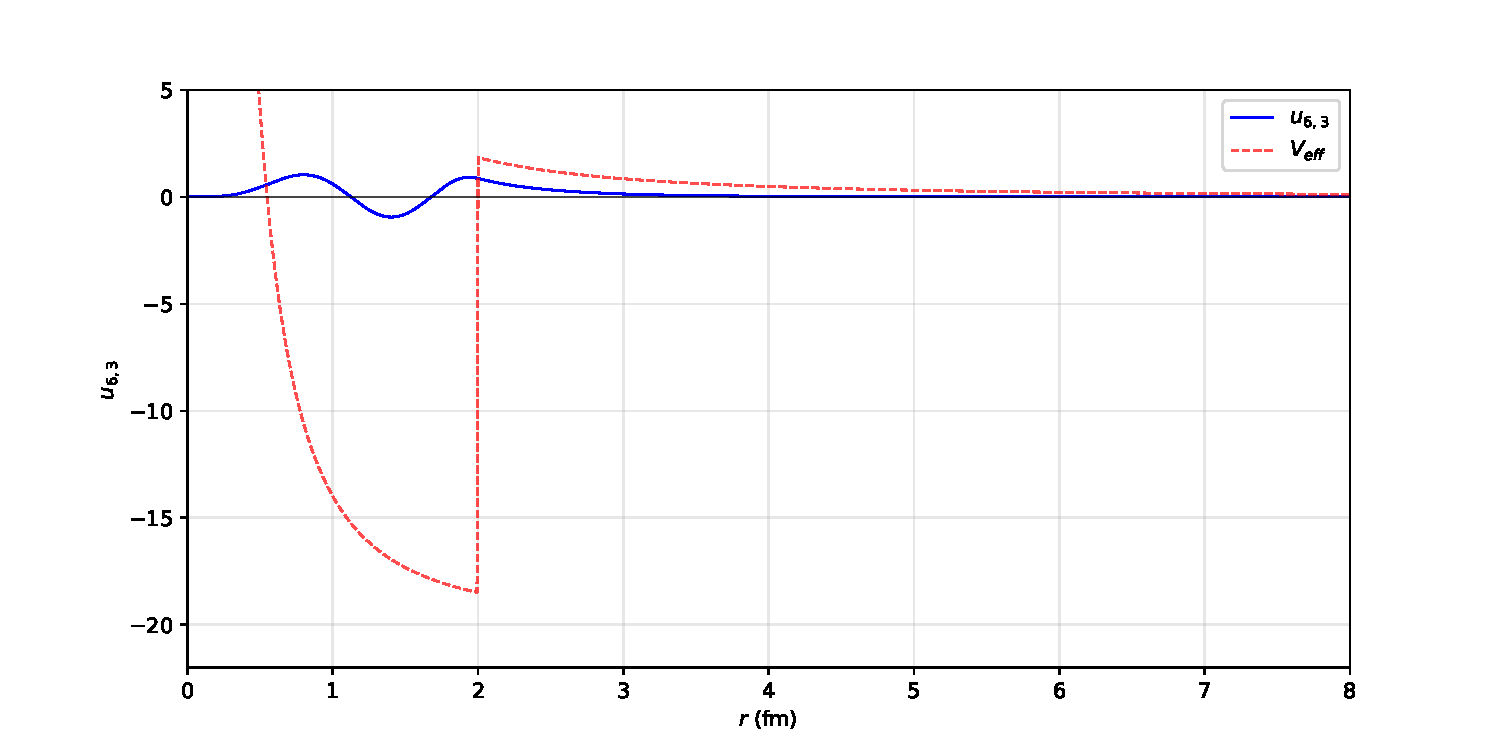
\includegraphics[width=\linewidth]{plots/wfs-and-pds/3/pb_wf_u63.pdf}
    \caption{Reduced radial wave function for $n = 6$, $\ell = 3$.}
    \label{fig:9}
  \end{figure}

  \begin{figure}[!htbp]
    \centering
    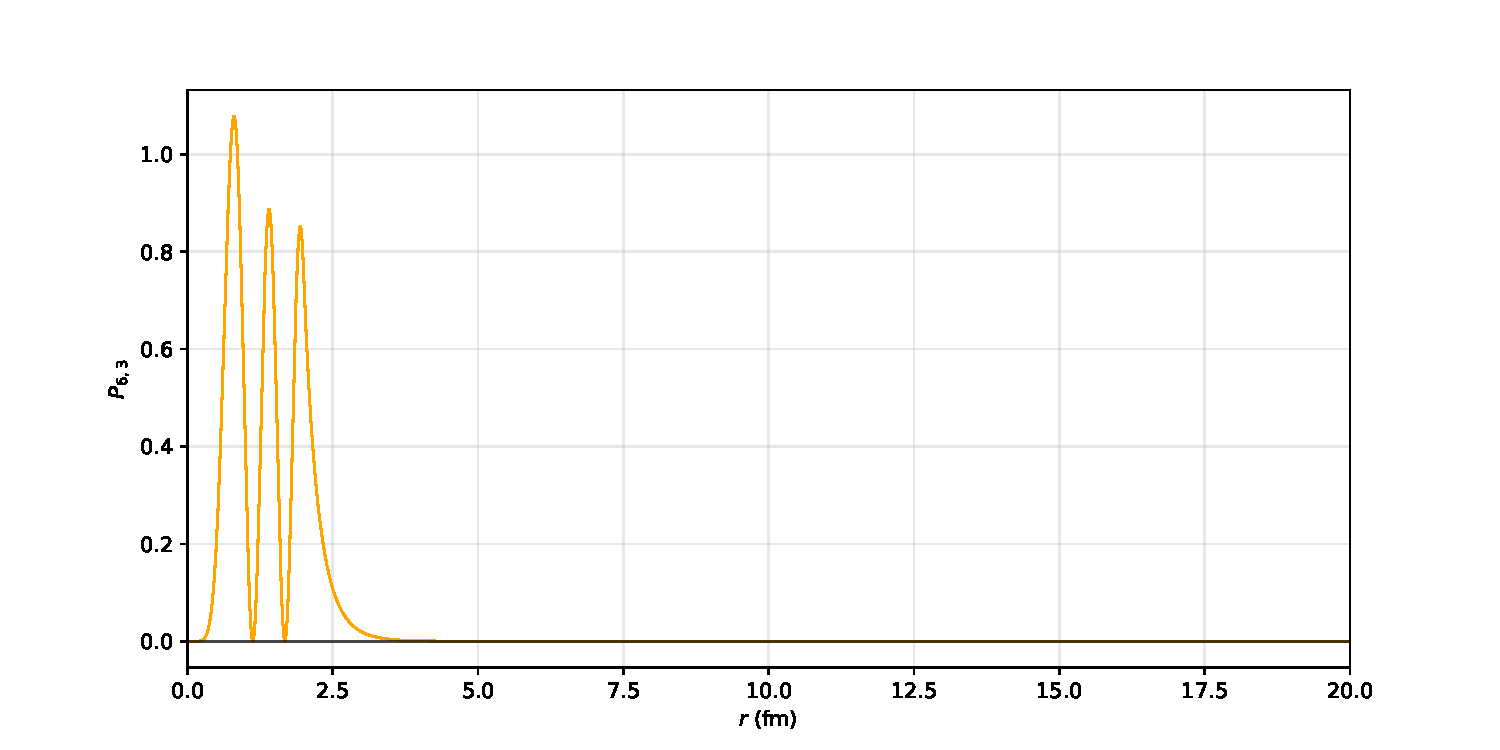
\includegraphics[width=\linewidth]{plots/wfs-and-pds/3/pb_pd_u63.pdf}
    \caption{Probability density $\mathcal{P}_{6,3}$ for $n = 6$, $\ell = 3$.}
    \label{fig:10}
  \end{figure}

  \begin{figure}[!htbp]
    \centering
    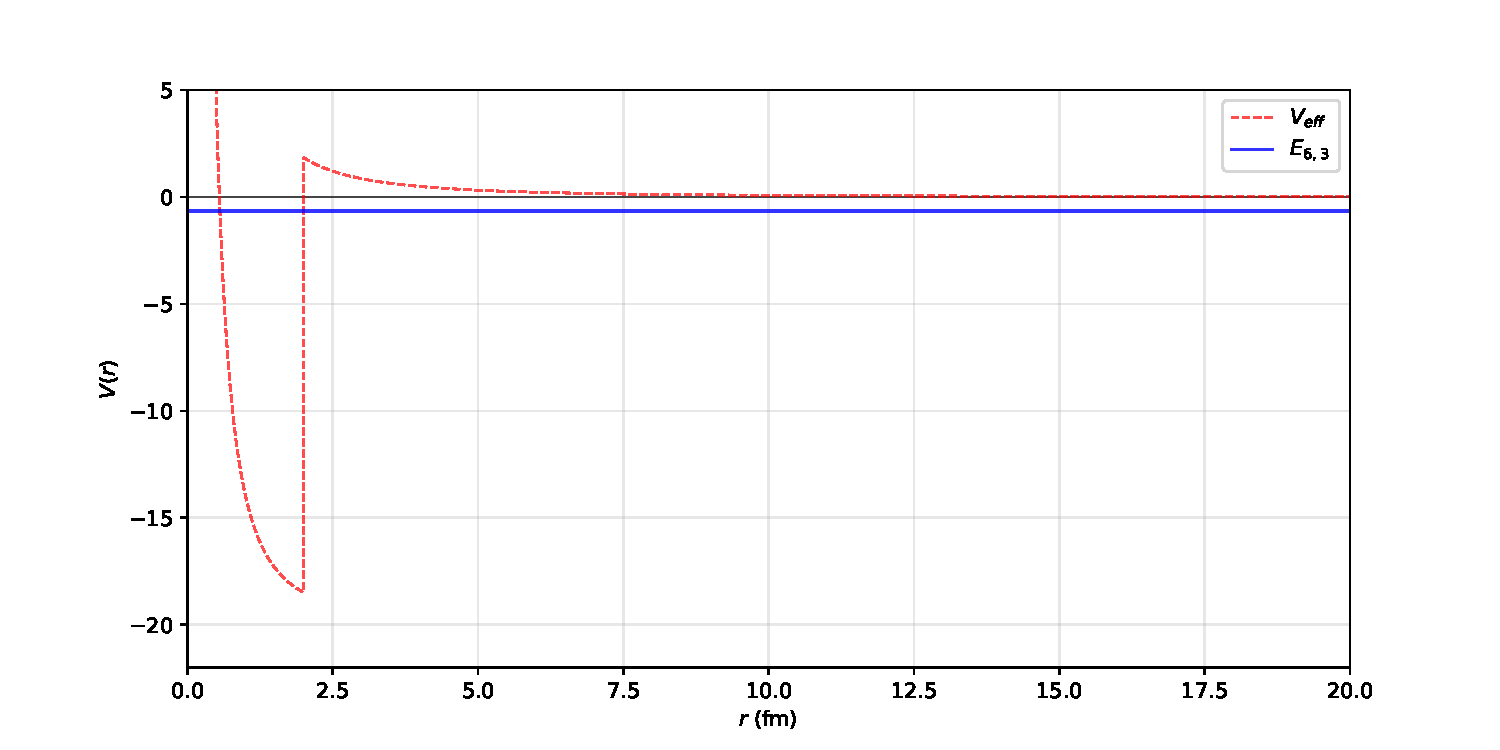
\includegraphics[width=\linewidth]{plots/energy/3/pb_pot_E63.pdf}
    \caption{Potential energy and total energy for $n = 6$, $\ell = 3$.}
    \label{fig:11}
  \end{figure}

  \begin{figure}[!htbp]
    \centering
    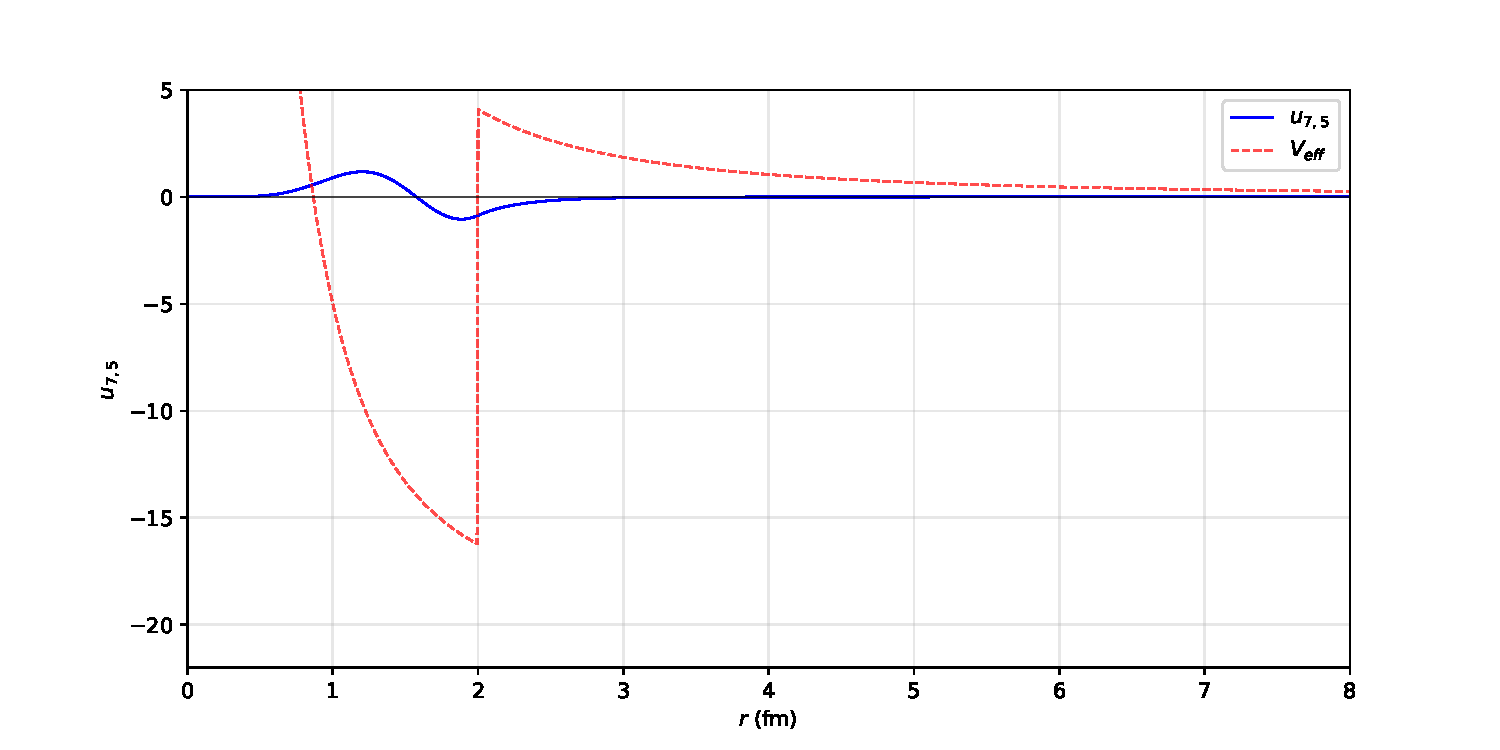
\includegraphics[width=\linewidth]{plots/wfs-and-pds/3/pb_wf_u75.pdf}
    \caption{Reduced radial wave function for $n = 7$, $\ell = 5$.}
    \label{fig:12}
  \end{figure}

  \begin{figure}[!htbp]
    \centering
    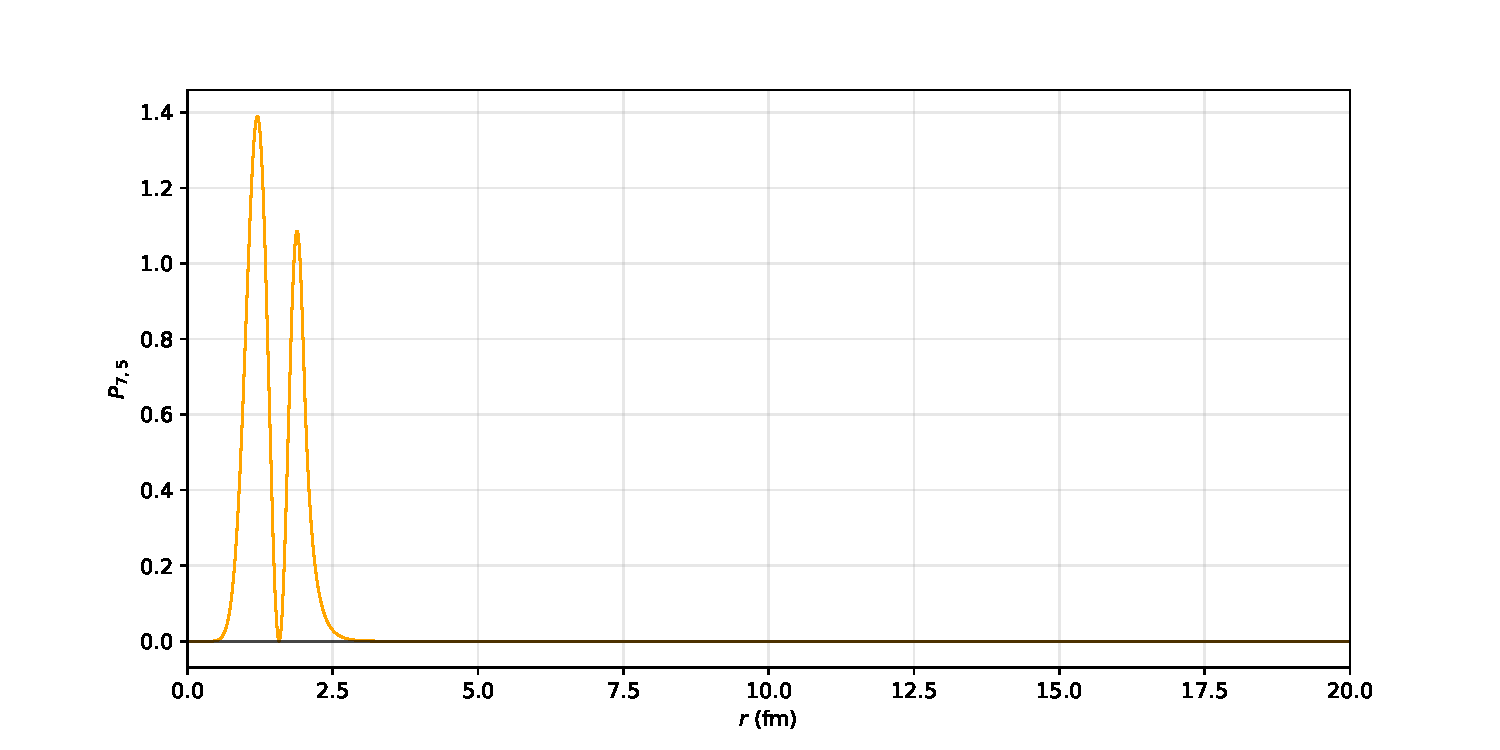
\includegraphics[width=\linewidth]{plots/wfs-and-pds/3/pb_pd_u75.pdf}
    \caption{Probability density $\mathcal{P}_{7,5}$ for $n = 7$, $\ell = 5$.}
    \label{fig:13}
  \end{figure}

  \begin{figure}[!htbp]
    \centering
    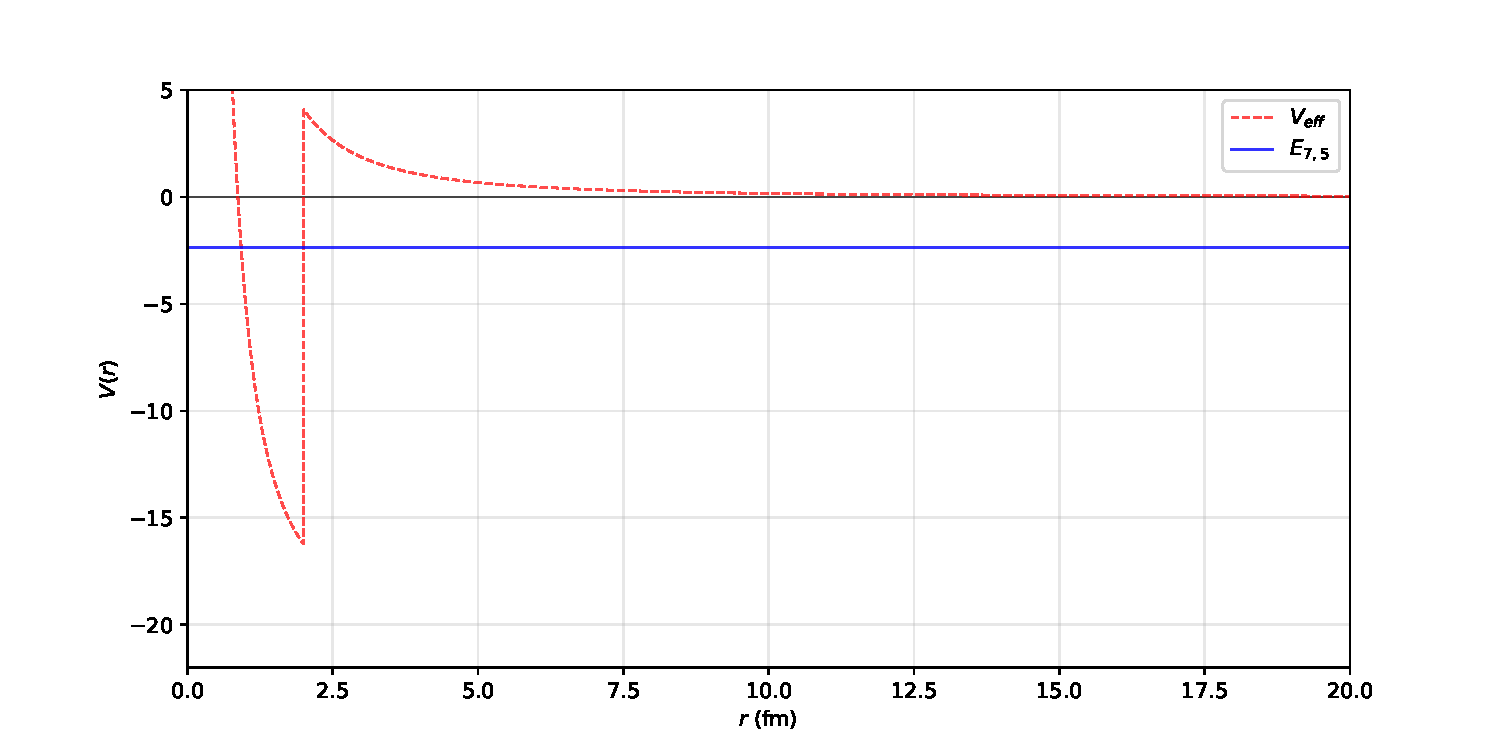
\includegraphics[width=\linewidth]{plots/energy/3/pb_pot_E75.pdf}
    \caption{Potential energy and total energy for $n = 7$, $\ell = 5$.}
    \label{fig:14}
  \end{figure}

  We now look at the $u_{25,5}$ state. 
  For the $u_{1,0}$, $u_{6,3}$, and $u_{7,5}$ states, the wave function decays towards zero as $r \rightarrow \infty$. 
  This is not the case for $u_{25,5}$, as it can be seen oscillating outside the region of the potential well in Fig. (\ref{fig:15}). 
  The reasoning behind this can be more easily inferred by looking at the state's probability distribution in Fig. (\ref{fig:16}). 

  \begin{figure}[!htbp]
    \centering
    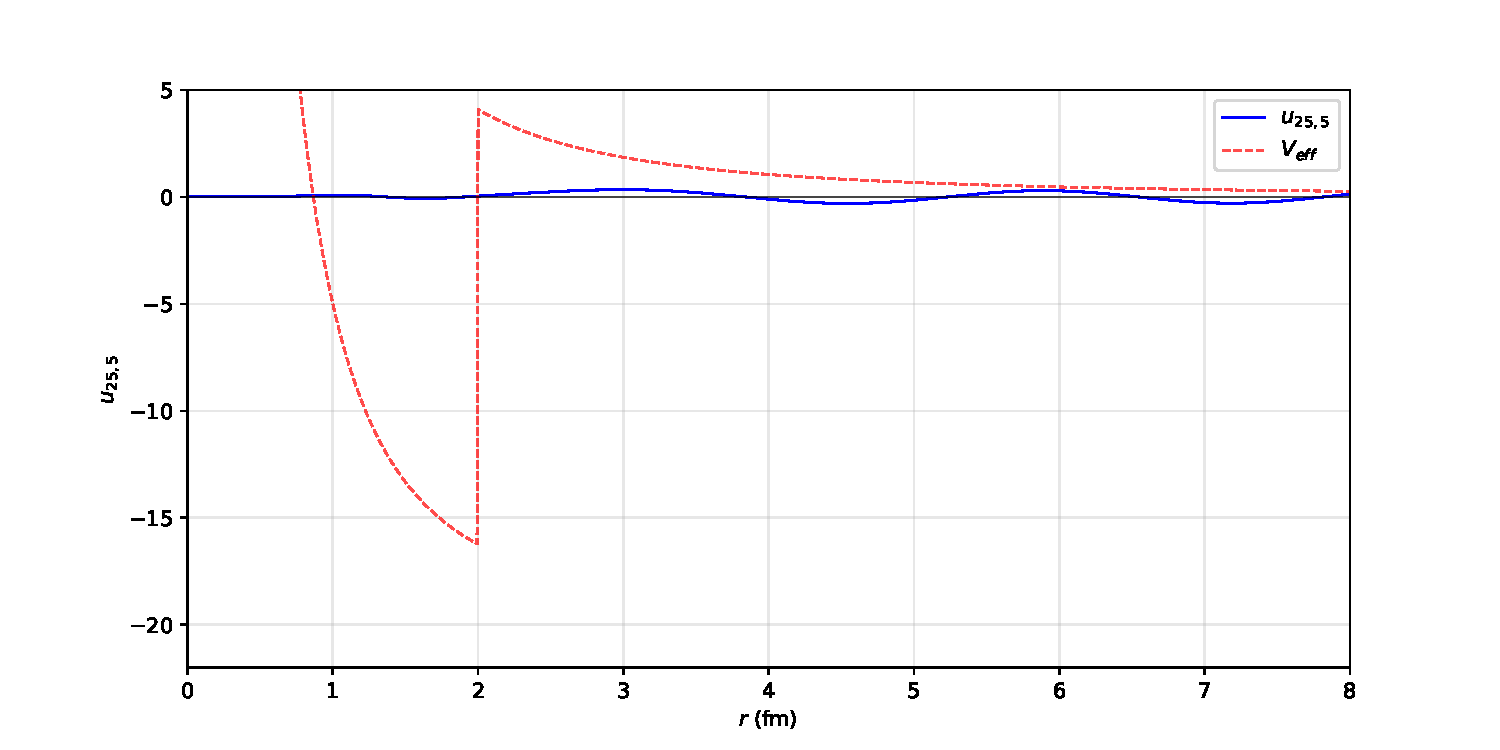
\includegraphics[width=\linewidth]{plots/wfs-and-pds/3/pb_wf_u255.pdf}
    \caption{Reduced radial wave function for $n = 25$, $\ell = 5$.}
    \label{fig:15}
  \end{figure}

  \begin{figure}[!htbp]
    \centering
    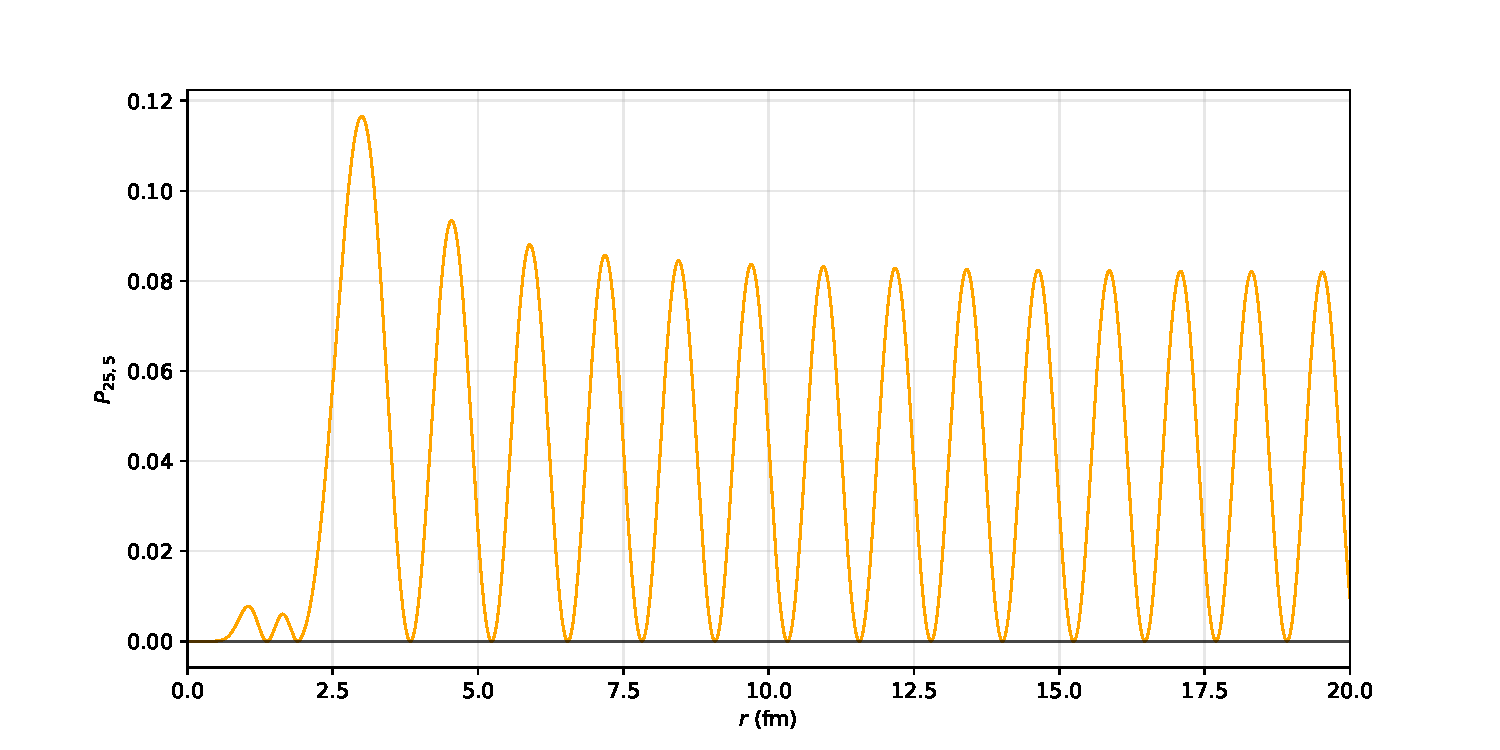
\includegraphics[width=\linewidth]{plots/wfs-and-pds/3/pb_pd_u255.pdf}
    \caption{Probability density $\mathcal{P}_{25,5}$ for $n = 25$, $\ell = 5$.}
    \label{fig:16}
  \end{figure}

  Clearly this is not a purely bound state; there is a high probability outside the well. 
  This is a scattering state. 
  We can look at the state's energy in comparison to the potential in Fig. (\ref{fig:17}).

  \begin{figure}[!htbp]
    \centering
    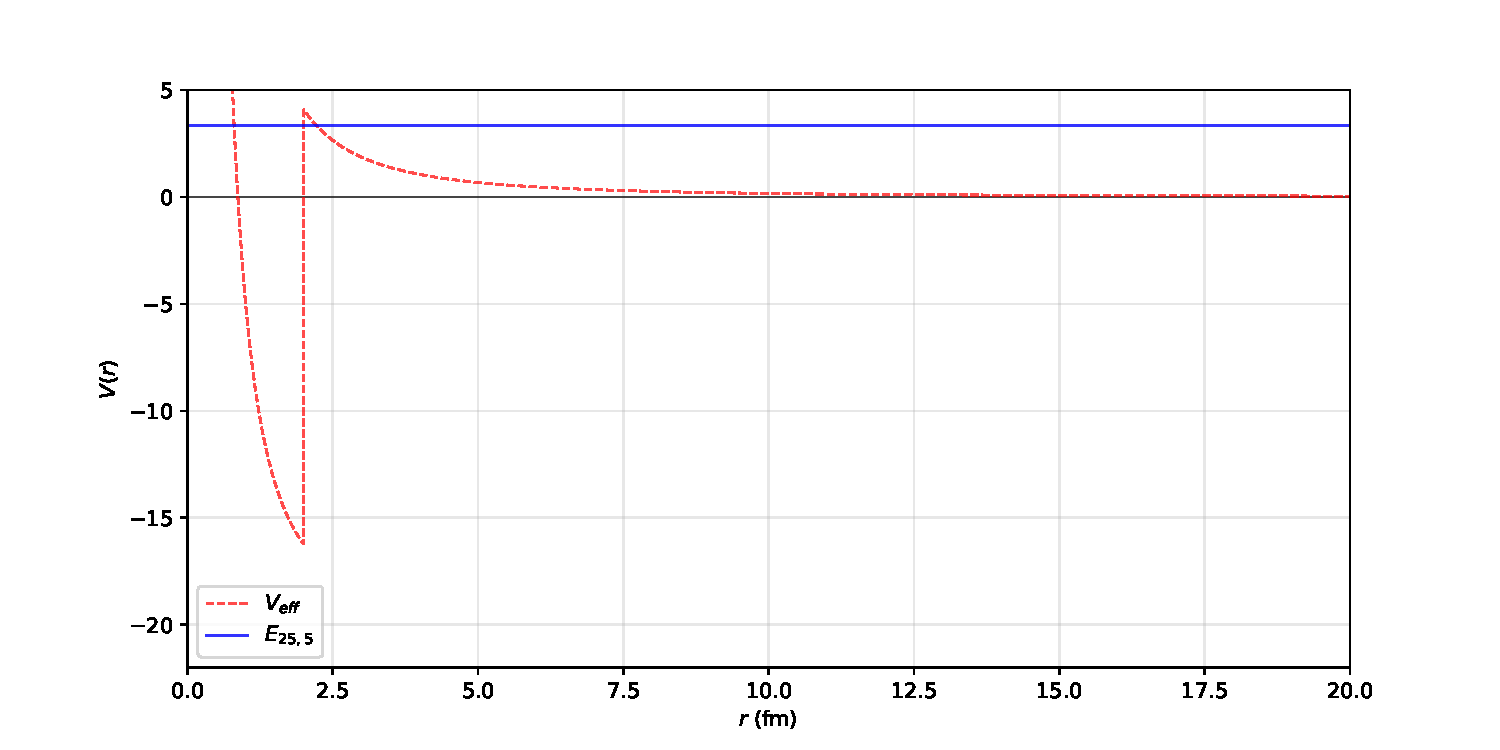
\includegraphics[width=\linewidth]{plots/energy/3/pb_pot_E255.pdf}
    \caption{Potential energy and total energy for $n = 25$, $\ell = 5$.}
    \label{fig:17}
  \end{figure}

  We can see the energy for this state is very close to the top of the well, allowing the wave function to ``leak'' through the potential, causing a tunneling effect. 

}
%\fi

%\fi % section


%\iffalse
% ====================
% Conclusions Section
% ====================
\section{\label{sec:conclusions}Conclusions}
{
  As seen from the results in App. (\ref{app:b}), as the radius of the spherical well $R$ increases, the number of bound states increase as well. 
  By looking at the difference\footnote{It is important to note the centrifugal potential does not change throughout these comparisons, only the pure Yukawa potential.} in potential in Figs. (\ref{fig:4}) and (\ref{fig:15}), we can see a clear difference in the allowed space a bound state can occupy. 
  In Fig. (\ref{fig:15}), we see how heavily the centrifugal term dominates, giving us a valid reason as to why the number of bound states would decrease. 
  We can use Fig. (\ref{fig:16}) as a visual aid, seeing just five bound states in this potential. 
  The jump in energy for $n$--states increases as well, with Fig. (\ref{fig:6}) showing $E_{20} \approx -16E^*$ and Fig. (\ref{fig:16}) showing $E_{20} \approx -6E^*$.
  We can also see the energies of pseudo-bound states increasing. 

  In App. (\ref{app:b}), we see how changing the well depth $V_0$ affects the number of bound states. 
  Though not as drastic a change as with the well width, the number of bound states decreases as well. 
  However, because the width of the well is still 2 fm, the contribution from the pure Yukawa potential doesn't stop the contribution from the centrifugal term as it did with $a = 1$ fm. 
  Therefore, the number of bound states decreases from the initial conditions, but not as much as it did when the width of the well decreased.

  App. (\ref{app:d}) shows the differences when $\lambda$ is changed, using $\lambda = 2.0$ and $\lambda = 10^{-5}$. 
  We can see as $\lambda \rightarrow 0$, the contribution to $V_{\text{eff}}$ gets bigger. 
  This is where the screening effect comes into play. 
  When $\lambda$ increases, as in Fig. (\ref{fig:51}), the Yukawa tail decays much quicker, therefore $V_{\text{eff}} \rightarrow V_{\text{Cent}}$ outside the region of the well. 
  
  The conclusions drawn from this exploratory project give further knowledge about concepts and understanding regarding nuclear physics, along with gaining computational experience. 
  Applying the use of computational methods allowed numerical modeling to be 
}
%\fi % section


%\iffalse
% =================
% Acknowledgements
% =================
\begin{acknowledgements}
{
  Acknowledgement towards the American Physical Society (APS) is warranted, as the format for this document is based on their template for APS articles. 
  Thank you to Dr. Alfa Heryudono for providing consultation throughout the process, for mathematical and computational support, as well as conceptual verification. 
  
}
\end{acknowledgements}
%\fi

% Bibliography: place here so it can sit at bottom of left column
\FloatBarrier
\nocite{*}  % cite all references (used & unused)
\bibliography{yuk-report}% Produces the bibliography via BibTeX.
% (removed \columnbreak — not defined for this class; appendix will follow)

% =========
% Appendix
% =========
\appendix

%\iffalse
% 
% 
% 
\section{\label{app:a}Total Energy with Potential Plots for $u_{1,0}$, $u_{6,3}$, and $u_{7,5}$.}
{
  \begin{figure}[!htbp]
    \centering
    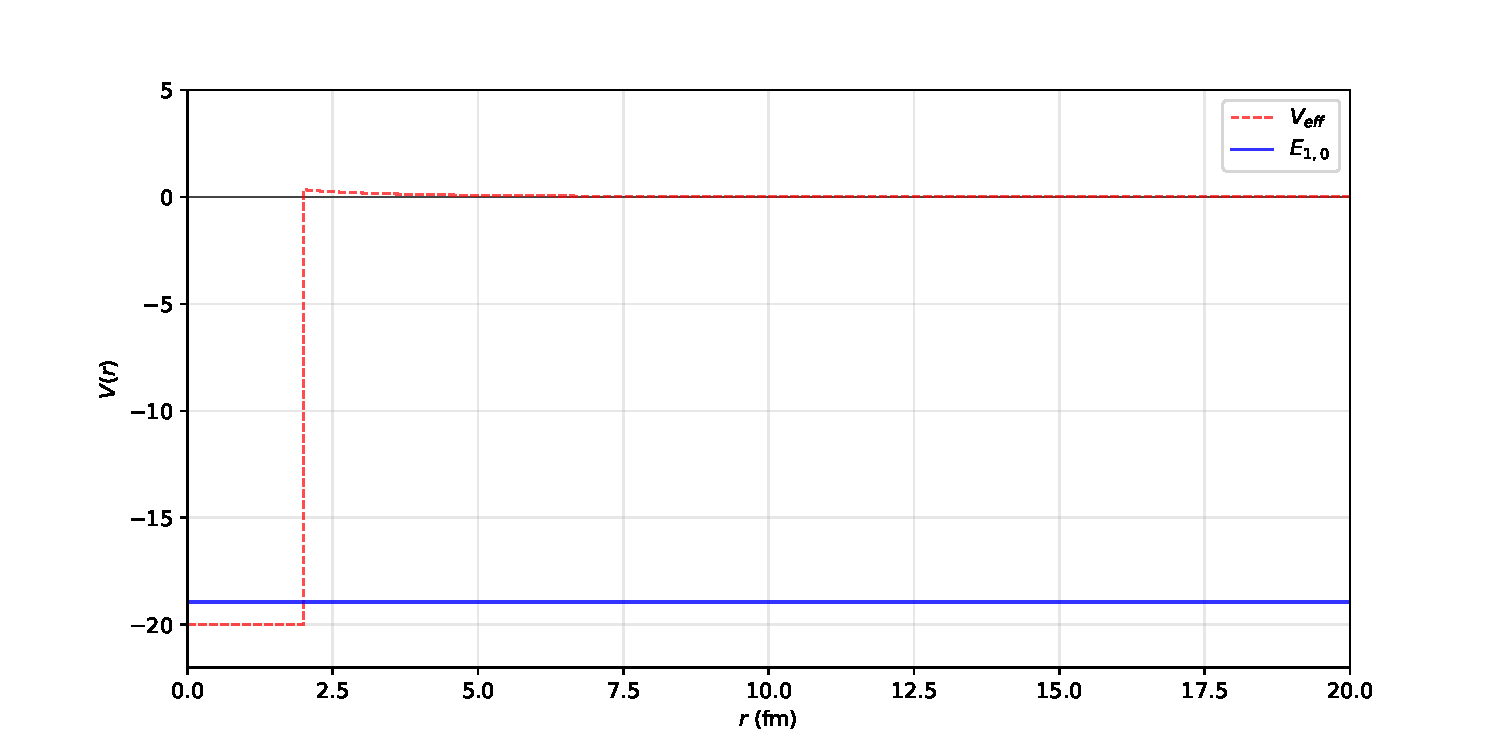
\includegraphics[width=\linewidth]{plots/energy/3/pb_pot_E10.pdf}
    \caption{Potential and total energy for $n = 1$, $\ell = 0$, the ground state.}
    \label{fig:18}
  \end{figure}

  \begin{figure}[!htbp]
    \centering
    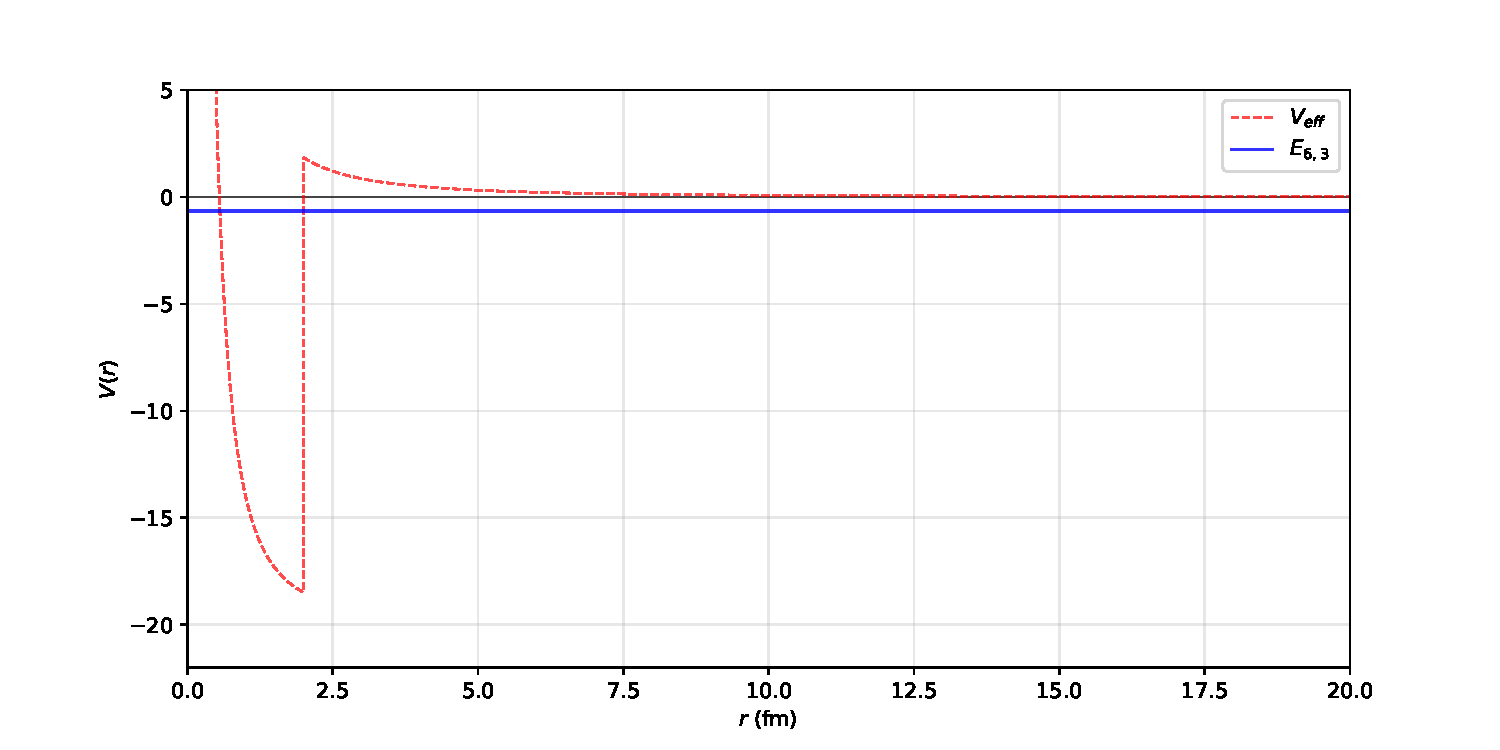
\includegraphics[width=\linewidth]{plots/energy/3/pb_pot_E63.pdf}
    \caption{Potential and total energy for $n = 6$, $\ell = 3$.}
    \label{fig:19}
  \end{figure}

  \begin{figure}[!htbp]
    \centering
    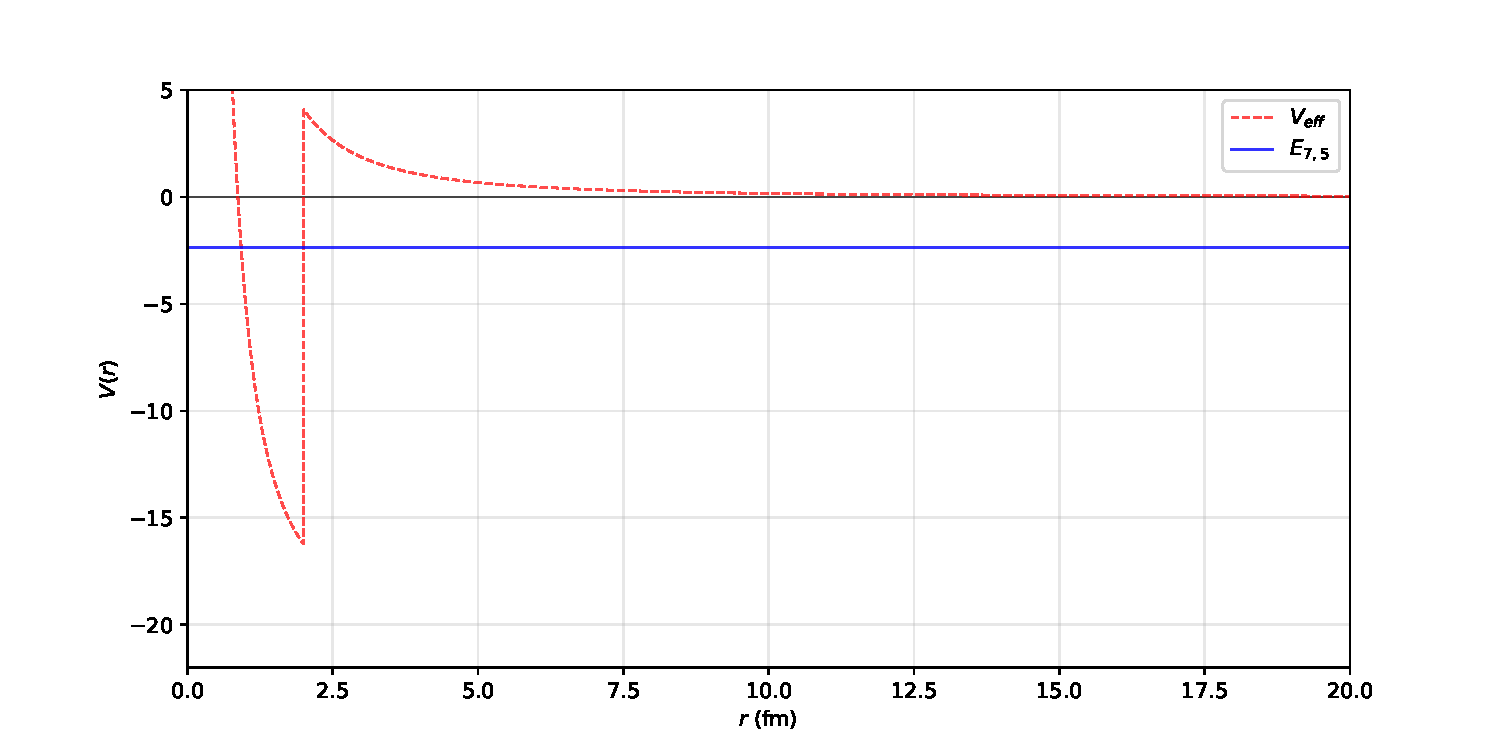
\includegraphics[width=\linewidth]{plots/energy/3/pb_pot_E75.pdf}
    \caption{Potential and total energy for $n = 7$, $\ell = 5$.}
    \label{fig:20}
  \end{figure}
}
%\fi

%\iffalse
% -----------------------
% Well Width: 2.0 -> 1.0
% -----------------------
\section{\label{app:b}Plot for Well Width $R = 1$ fm}
{
  These plots are the product of only changing $R$ from the initial parameters. 
  All other parameters remain the same, with $R = 1 \text{ fm}$, $\lambda = 0.2$, $V_0 = 20 E^*$. 
  See: 
  \begin{enumerate}%[label=(\alph*)]
    \item Potential $V(r)$ -- \ref{fig:21}
    \item Energy $E$ -- \ref{fig:22}
    \item $n = 1$, $\ell = 0$ -- \ref{fig:23}
    \item $n = 6$, $\ell = 3$ -- \ref{fig:26}
    \item $n = 7$, $\ell = 5$ -- \ref{fig:29}
    \item $n = 25$, $\ell = 5$ -- \ref{fig:32}
  \end{enumerate}

  \begin{figure}[!htbp]
    \centering
    
\includegraphics[width=\linewidth]{plots/potential/4/pb_Vr_L5.pdf}
    \caption{Effective Yukawa potential for $\ell = 5$ ($R = 1$ fm).}
    \label{fig:21}
  \end{figure}

  \begin{figure}[!htbp]
    \centering
    
\includegraphics[width=\linewidth]{plots/energy/4/pb_energy.pdf}
    \caption{Yukawa energy from $\ell = 0$ to $\ell = 5$ ($R = 1$ fm).}
    \label{fig:22}
  \end{figure}

  \begin{figure}[!htbp]
    \centering
    
\includegraphics[width=\linewidth]{plots/wfs-and-pds/4/pb_wf_u10.pdf}
    \caption{Reduced radial wave function for $n = 1$, $\ell = 0$, the ground state ($R = 1$ fm).}
    \label{fig:23}
  \end{figure}

  \begin{figure}[!htbp]
    \centering
    
\includegraphics[width=\linewidth]{plots/wfs-and-pds/4/pb_pd_u10.pdf}
    \caption{Probability density $\mathcal{P}_{10}$ for $n = 1$, $\ell = 0$, the ground state ($R = 1$ fm).}
    \label{fig:24}
  \end{figure}
  
  \begin{figure}[!htbp]
    \centering
    
\includegraphics[width=\linewidth]{plots/energy/4/pb_pot_E10.pdf}
    \caption{Potential and total energy for $n = 1$, $\ell = 0$, the ground state.}
    \label{fig:25}
  \end{figure}
  
  \begin{figure}[!htbp]
    \centering
    
\includegraphics[width=\linewidth]{plots/wfs-and-pds/4/pb_wf_u63.pdf}
    \caption{Reduced radial wave function for $n = 6$, $\ell = 3$ ($R = 1$ fm).}
    \label{fig:26}
  \end{figure}

  \begin{figure}[!htbp]
    \centering
    
\includegraphics[width=\linewidth]{plots/wfs-and-pds/4/pb_pd_u63.pdf}
    \caption{Probability density $\mathcal{P}_{6,3}$ for $n = 6$, $\ell = 3$ ($R = 1$ fm).}
    \label{fig:27}
  \end{figure}

  \begin{figure}[!htbp]
    \centering
    
\includegraphics[width=\linewidth]{plots/energy/4/pb_pot_E63.pdf}
    \caption{Potential and total energy for $n = 6$, $\ell = 3$.}
    \label{fig:28}
  \end{figure}

  \begin{figure}[!htbp]
    \centering
    
\includegraphics[width=\linewidth]{plots/wfs-and-pds/4/pb_wf_u75.pdf}
    \caption{Reduced radial wave function for $n = 7$, $\ell = 5$ ($R = 1$ fm).}
    \label{fig:29}
  \end{figure}

  \begin{figure}[!htbp]
    \centering
    
\includegraphics[width=\linewidth]{plots/wfs-and-pds/4/pb_pd_u75.pdf}
    \caption{Probability density $\mathcal{P}_{7,5}$ for $n = 7$, $\ell = 5$ ($R = 1$ fm).}
    \label{fig:30}
  \end{figure}

  \begin{figure}[!htbp]
    \centering
    
\includegraphics[width=\linewidth]{plots/energy/4/pb_pot_E75.pdf}
    \caption{Potential and total energy for $n = 7$, $\ell = 5$.}
    \label{fig:31}
  \end{figure}

  \begin{figure}[!htbp]
    \centering
    
\includegraphics[width=\linewidth]{plots/wfs-and-pds/4/pb_wf_u255.pdf}
    \caption{Reduced radial wave function for $n = 25$, $\ell = 5$ ($R = 1$ fm).}
    \label{fig:32}
  \end{figure}

  \begin{figure}[!htbp]
    \centering
    
\includegraphics[width=\linewidth]{plots/wfs-and-pds/4/pb_pd_u255.pdf}
    \caption{Probability density $\mathcal{P}_{25,5}$ for $n = 25$, $\ell = 5$ ($R = 1$ fm).}
    \label{fig:33}
  \end{figure}

  \begin{figure}[!htbp]
    \centering
    
\includegraphics[width=\linewidth]{plots/energy/4/pb_pot_E255.pdf}
    \caption{Potential and total energy for $n = 25$, $\ell = 5$.}
    \label{fig:34}
  \end{figure}
}
%\FloatBarrier
%\fi

%\iffalse
% -------------------------
% Well Depth: 20.0 -> 10.0
% -------------------------
\section{\label{app:c}Plots for Well Depth $V_0 = 10E^*$}
{
  These plots are the product of only changing $V_0$ from the initial parameters. 
  All other parameters remain the same, with $R = 2 \text{ fm}$, $\lambda = 0.2$, $V_0 = 10 E^*$. 
  See: 

  \begin{enumerate}%[label=(\alph*)]
    \item Potential $V(r)$ -- \ref{fig:21}
    \item Energy $E$ -- \ref{fig:22}
    \item $n = 1$, $\ell = 0$ -- \ref{fig:37}
    \item $n = 6$, $\ell = 3$ -- \ref{fig:40}
    \item $n = 7$, $\ell = 5$ -- \ref{fig:43}
    \item $n = 25$, $\ell = 5$ -- \ref{fig:46}
  \end{enumerate}

  \begin{figure}[!htbp]
    \centering
    
\includegraphics[width=\linewidth]{plots/potential/5/pb_Vr_L5.pdf}
    \caption{Effective Yukawa potential for $\ell = 5$ ($V_0 = 10E^*$).}
    \label{fig:35}
  \end{figure}

  \begin{figure}[!htbp]
    \centering
    
\includegraphics[width=\linewidth]{plots/energy/5/pb_energy.pdf}
    \caption{Yukawa energy from $\ell = 0$ to $\ell = 5$ ($V_0 = 10E^*$).}
    \label{fig:36}
  \end{figure}  

\begin{figure}[!htbp]
    \centering
    
\includegraphics[width=\linewidth]{plots/wfs-and-pds/5/pb_wf_u10.pdf}
    \caption{Reduced radial wave function for $n = 1$, $\ell = 0$, the ground state ($V_0 = 10E^*$).}
    \label{fig:37}
  \end{figure}

  \begin{figure}[!htbp]
    \centering
    
\includegraphics[width=\linewidth]{plots/wfs-and-pds/5/pb_pd_u10.pdf}
    \caption{Probability density $\mathcal{P}_{10}$ for $n = 1$, $\ell = 0$, the ground state ($V_0 = 10E^*$).}
    \label{fig:38}
  \end{figure}

  
  \begin{figure}[!htbp]
    \centering
    
\includegraphics[width=\linewidth]{plots/energy/5/pb_pot_E10.pdf}
    \caption{Potential and total energy for $n = 1$, $\ell = 0$, the ground state.}
    \label{fig:39}
  \end{figure}
  

  \begin{figure}[!htbp]
    \centering
    
\includegraphics[width=\linewidth]{plots/wfs-and-pds/5/pb_wf_u63.pdf}
    \caption{Reduced radial wave function for $n = 6$, $\ell = 3$ ($V_0 = 10E^*$).}
    \label{fig:40}
  \end{figure}

  \begin{figure}[!htbp]
    \centering
    
\includegraphics[width=\linewidth]{plots/wfs-and-pds/5/pb_pd_u63.pdf}
    \caption{Probability density $\mathcal{P}_{6,3}$ for $n = 6$, $\ell = 3$ ($V_0 = 10E^*$).}
    \label{fig:41}
  \end{figure}

  \begin{figure}[!htbp]
    \centering
    
\includegraphics[width=\linewidth]{plots/energy/5/pb_pot_E63.pdf}
    \caption{Potential and total energy for $n = 6$, $\ell = 3$.}
    \label{fig:42}
  \end{figure}

  \begin{figure}[!htbp]
    \centering
    
\includegraphics[width=\linewidth]{plots/wfs-and-pds/5/pb_wf_u75.pdf}
    \caption{Reduced radial wave function for $n = 7$, $\ell = 5$ ($V_0 = 10E^*$).}
    \label{fig:43}
  \end{figure}

  \begin{figure}[!htbp]
    \centering
    
\includegraphics[width=\linewidth]{plots/wfs-and-pds/5/pb_pd_u75.pdf}
    \caption{Probability density $\mathcal{P}_{7,5}$ for $n = 7$, $\ell = 5$ ($V_0 = 10E^*$).}
    \label{fig:44}
  \end{figure}

  \begin{figure}[!htbp]
    \centering
    
\includegraphics[width=\linewidth]{plots/energy/5/pb_pot_E75.pdf}
    \caption{Potential and total energy for $n = 7$, $\ell = 5$.}
    \label{fig:45}
  \end{figure}

  \begin{figure}[!htbp]
    \centering
    
\includegraphics[width=\linewidth]{plots/wfs-and-pds/5/pb_wf_u255.pdf}
    \caption{Reduced radial wave function for $n = 25$, $\ell = 5$ ($V_0 = 10E^*$).}
    \label{fig:46}
  \end{figure}

  \begin{figure}[!htbp]
    \centering
    
\includegraphics[width=\linewidth]{plots/wfs-and-pds/5/pb_pd_u255.pdf}
    \caption{Probability density $\mathcal{P}_{25,5}$ for $n = 25$, $\ell = 5$ ($V_0 = 10E^*$).}
    \label{fig:47}
  \end{figure}

  \begin{figure}[!htbp]
    \centering
    
\includegraphics[width=\linewidth]{plots/energy/5/pb_pot_E255.pdf}
    \caption{Potential and total energy for $n = 25$, $\ell = 5$.}
    \label{fig:48}
  \end{figure}
}
%\FloatBarrier
%\enlargethispage{2\baselineskip}
%\fi

%\iffalse
% ----------------------------------------------
% Screening Parameter: \lambda -> {2.0, 0.0001}
% ----------------------------------------------
\section{\label{app:d}Plots for Screening Parameter $\lambda = 2.0, 10^{-5}$}
{
  These plots are the product of only changing $\lambda$ from the initial parameters. 
  All other parameters remain the same, with $R = 2 \text{ fm}$, $\lambda = 0.2, 10^{-5}$, $V_0 = 20 E^*$. 
  See: 
  \begin{enumerate}%[label=(\alph*)]
    \item Potential $V(r)$ -- \ref{fig:49}
    \item Energy $E$ -- \ref{fig:51}
    \item $n = 1$, $\ell = 0$ -- \ref{fig:53}
    \item $n = 6$, $\ell = 3$ -- \ref{fig:59}
    \item $n = 7$, $\ell = 5$ -- \ref{fig:65}
    \item $n = 25$, $\ell = 5$ -- \ref{fig:71}
  \end{enumerate}

  \begin{figure}[!htbp]
    \centering
    
\includegraphics[width=\linewidth]{plots/energy/6/pb_energy.pdf}
    \caption{Yukawa energy from $\ell = 0$ to $\ell = 5$ ($\lambda = 2$).}
    \label{fig:49}
  \end{figure}

  \begin{figure}[!htbp]
    \centering
    
\includegraphics[width=\linewidth]{plots/energy/7/pb_energy.pdf}
    \caption{Yukawa energy from $\ell = 0$ to $\ell = 5$ ($\lambda = 10^{-5}$).}
    \label{fig:50}
  \end{figure}

  \begin{figure}[!htbp]
    \centering
    
\includegraphics[width=\linewidth]{plots/potential/6/pb_Vr_L5.pdf}
    \caption{Effective Yukawa potential for $\ell = 5$ ($\lambda = 2$).}
    \label{fig:51}
  \end{figure}

  \begin{figure}[!htbp]
    \centering
    
\includegraphics[width=\linewidth]{plots/potential/7/pb_Vr_L5.pdf}
    \caption{Effective Yukawa potential for $\ell = 5$ ($\lambda = 10^{-5}$).}
    \label{fig:52}
  \end{figure}
  
  \begin{figure}[!htbp]
    \centering
    
\includegraphics[width=\linewidth]{plots/wfs-and-pds/6/pb_wf_u10.pdf}
    \caption{Reduced radial wave function for $n = 1$, $\ell = 0$, the ground state ($\lambda = 2$).}
    \label{fig:53}
  \end{figure}

  \begin{figure}[!htbp]
    \centering
    
\includegraphics[width=\linewidth]{plots/wfs-and-pds/7/pb_wf_u10.pdf}
    \caption{Reduced radial wave function for $n = 1$, $\ell = 0$, the ground state ($\lambda = 10^{-5}$).}
    \label{fig:54}
  \end{figure}

  \begin{figure}[!htbp]
    \centering
    
\includegraphics[width=\linewidth]{plots/wfs-and-pds/6/pb_pd_u10.pdf}
    \caption{Probability density $\mathcal{P}_{10}$ for $n = 1$, $\ell = 0$, the ground state ($\lambda = 2$).}
    \label{fig:55}
  \end{figure}
  
  \begin{figure}[!htbp]
    \centering
    
\includegraphics[width=\linewidth]{plots/wfs-and-pds/7/pb_pd_u10.pdf}
    \caption{Probability density $\mathcal{P}_{10}$ for $n = 1$, $\ell = 0$, the ground state ($\lambda = 10^{-5}$).}
    \label{fig:56}
  \end{figure}

  
  \begin{figure}[!htbp]
    \centering
    
\includegraphics[width=\linewidth]{plots/energy/6/pb_pot_E10.pdf}
    \caption{Potential and total energy for $n = 1$, $\ell = 0$, the ground state ($\lambda = 2$).}
    \label{fig:57}
  \end{figure}

  \begin{figure}[!htbp]
    \centering
    
\includegraphics[width=\linewidth]{plots/energy/7/pb_pot_E10.pdf}
    \caption{Potential and total energy for $n = 1$, $\ell = 0$, the ground state ($\lambda = 10^{-5}$).}
    \label{fig:58}
  \end{figure}
  

  \begin{figure}[!htbp]
    \centering
    
\includegraphics[width=\linewidth]{plots/wfs-and-pds/6/pb_wf_u63.pdf}
    \caption{Reduced radial wave function for $n = 6$, $\ell = 3$ ($\lambda = 2$).}
    \label{fig:59}
  \end{figure}

  \begin{figure}[!htbp]
    \centering
    
\includegraphics[width=\linewidth]{plots/wfs-and-pds/7/pb_wf_u63.pdf}
    \caption{Reduced radial wave function for $n = 6$, $\ell = 3$ ($\lambda = 10^{-5}$).}
    \label{fig:60}
  \end{figure}
  
  \begin{figure}[!htbp]
    \centering
    
\includegraphics[width=\linewidth]{plots/wfs-and-pds/6/pb_pd_u63.pdf}
    \caption{Probability density $\mathcal{P}_{6,3}$ for $n = 6$, $\ell = 3$ ($\lambda = 2$).}
    \label{fig:61}
  \end{figure}

  \begin{figure}[!htbp]
    \centering
    
\includegraphics[width=\linewidth]{plots/wfs-and-pds/7/pb_pd_u63.pdf}
    \caption{Probability density $\mathcal{P}_{6,3}$ for $n = 6$, $\ell = 3$ ($\lambda = 10^{-5}$).}
    \label{fig:62}
  \end{figure}

    \begin{figure}[!htbp]
    \centering
    
\includegraphics[width=\linewidth]{plots/energy/6/pb_pot_E63.pdf}
    \caption{Potential and total energy for $n = 6$, $\ell = 3$ ($\lambda = 2$).}
    \label{fig:63}
  \end{figure}

  \begin{figure}[!htbp]
    \centering
    
\includegraphics[width=\linewidth]{plots/energy/7/pb_pot_E63.pdf}
    \caption{Potential and total energy for $n = 6$, $\ell = 3$ ($\lambda = 10^{-5}$).}
    \label{fig:64}
  \end{figure}

  \begin{figure}[!htbp]
    \centering
    
\includegraphics[width=\linewidth]{plots/wfs-and-pds/6/pb_wf_u75.pdf}
    \caption{Reduced radial wave function for $n = 7$, $\ell = 5$ ($\lambda = 2$).}
    \label{fig:65}
  \end{figure}

  \begin{figure}[!htbp]
    \centering
    
\includegraphics[width=\linewidth]{plots/wfs-and-pds/7/pb_wf_u75.pdf}
    \caption{Reduced radial wave function for $n = 7$, $\ell = 5$ ($\lambda = 10^{-5}$).}
    \label{fig:66}
  \end{figure}

  \begin{figure}[!htbp]
    \centering
    
\includegraphics[width=\linewidth]{plots/wfs-and-pds/6/pb_pd_u75.pdf}
    \caption{Probability density $\mathcal{P}_{7,5}$ for $n = 7$, $\ell = 5$ ($\lambda = 2$).}
    \label{fig:67}
  \end{figure}
  
  \begin{figure}[!htbp]
    \centering
    
\includegraphics[width=\linewidth]{plots/wfs-and-pds/7/pb_pd_u75.pdf}
    \caption{Probability density $\mathcal{P}_{7,5}$ for $n = 7$, $\ell = 5$ ($\lambda = 10^{-5}$).}
    \label{fig:68}
  \end{figure}

  \begin{figure}[!htbp]
    \centering
    
\includegraphics[width=\linewidth]{plots/energy/6/pb_pot_E75.pdf}
    \caption{Potential and total energy for $n = 7$, $\ell = 5$ ($\lambda = 2$).}
    \label{fig:69}
  \end{figure}

  \begin{figure}[!htbp]
    \centering
    
\includegraphics[width=\linewidth]{plots/energy/7/pb_pot_E75.pdf}
    \caption{Potential and total energy for $n = 7$, $\ell = 5$ ($\lambda = 10^{-5}$).}
    \label{fig:70}
  \end{figure}

  \begin{figure}[!htbp]
    \centering
    
\includegraphics[width=\linewidth]{plots/wfs-and-pds/6/pb_wf_u255.pdf}
    \caption{Reduced radial wave function for $n = 25$, $\ell = 5$ ($\lambda = 2$).}
    \label{fig:71}
  \end{figure}

  \begin{figure}[!htbp]
    \centering
    
\includegraphics[width=\linewidth]{plots/wfs-and-pds/7/pb_wf_u255.pdf}
    \caption{Reduced radial wave function for $n = 25$, $\ell = 5$ ($\lambda = 10^{-5}$).}
    \label{fig:72}
  \end{figure}
  
  \begin{figure}[!htbp]
    \centering
    
\includegraphics[width=\linewidth]{plots/wfs-and-pds/6/pb_pd_u255.pdf}
    \caption{Probability density $\mathcal{P}_{25,5}$ for $n = 25$, $\ell = 5$ ($\lambda = 2$).}
    \label{fig:73}
  \end{figure}

  \begin{figure}[!htbp]
    \centering
    
\includegraphics[width=\linewidth]{plots/wfs-and-pds/7/pb_pd_u255.pdf}
    \caption{Probability density $\mathcal{P}_{25,5}$ for $n = 25$, $\ell = 5$ ($\lambda = 10^{-5}$).}
    \label{fig:74}
  \end{figure}

  \begin{figure}[!htbp]
    \centering
    
\includegraphics[width=\linewidth]{plots/energy/6/pb_pot_E255.pdf}
    \caption{Potential and total energy for $n = 25$, $\ell = 5$ ($\lambda = 2$).}
    \label{fig:75}
  \end{figure}

  \begin{figure}[!htbp]
    \centering
    
\includegraphics[width=\linewidth]{plots/energy/7/pb_pot_E255.pdf}
    \caption{Potential and total energy for $n = 25$, $\ell = 5$ ($\lambda = 10^{-5}$).}
    \label{fig:76}
  \end{figure}
}
%\FloatBarrier
\end{document}
